% !TeX spellcheck = en
\chapter{Implementation}
\label{sec:impl}
This chapter presents the steps of development and implementation of the proposed approach. The Unity Application for HoloLens was deployed on HMD and raw data with measures and dimension columns was obtained. This data was analysed and preprocessed to ensure that the captured data can be used in corresponding machine learning models. The model architecture was implemented and experimentally improved during training and evaluation steps.

\section{6-DoF Dataset}
\label{sec:impl:dataset}
This section describes how the dataset was obtained, analysed and presents the visualisation of the user's head position and rotation. Almost all machine learning approaches require not only row data collection but also data exploration and preprocessing steps to be done before training begins.

\subsection{Data collection from HMD}
\label{sec:impl:dataset:HL}
The real 6-DoF dataset must be used as training data from which the model can learn the spatial and time dependencies. In this master thesis HoloLens 2, the second iteration of Microsoft's head-mounted mixed reality device, was used for data collection. The user position and orientation were obtained with the Unity application developed for this purpose. The Main Camera in Unity is automatically configured to track head movements. More details about Unity application can be found in section \ref{sec:impl:model:dev:unity}. Using the Main Camera, a user position $(x, y, z)$ and orientation in quaternion $(qx, qy, qz, qw)$ were logged in a $csv$-file. Quaternions obtained from HMD will be used to define a rotation by four numbers. Quaternion representations are very convenient for operations such as composition or rotations and coordinate transformation \cite{principles_robot_motion_book}. For these reasons quaternions are chosen for the representation of the user head's rotation in three dimensions. Compared to the dataset in \cite{serhan_kalman}, the additional parameters were recorded from the Main Camera in order to add more information during training processes. Thus the world-space speed of the camera in metres per second was recorded. Unity velocity has the speed in $(x, y, z)$ defining the direction. The obtained 6-DoF dataset has 10 features used in the training process: position $(x, y, z)$, orientation $(qx, qy, qz, qw)$ and velocity $(x, y, z)$.

The datasets were recorded in the laboratory space. HMD was presented to users and the basic functions were explained. During data recording, users freely walked wearing HMD in laboratory space. The Unity application, running on HMD, not only recorded the mentioned parameters but also had a volumetric animated object placed 3 metres ahead of the user in the Mixed Reality environment. No personal data was recorded during these sessions and all traces are obtained anonymously. Thus, after an Unity application was launched, users could immediately see the animated object. The several traces were recorded for at least 10 minutes each. It allows to have enough data after splitting the dataset into training, test and validation partitions. Table \ref{tab:raw_data} show the first 20 rows from the raw dataset obtained from HoloLens 2 and used in training. Although the dataset has 10 columns, the table \ref{tab:raw_data} presents only $timestamp$ and position $(x, y, z)$ columns. 

\begin{table}[!ht]
		\footnotesize
		\centering
	\begin{tabular}{|l|l|l|l|}
		\hline
		timestamp & x & y & z \\ [0.5ex] 
		\hline\hline
		2.649431 & 0.004954389 & 0.003402365 & 0.01010712 \\ \hline
		2.66943 & 0.00459053 & 0.003120769 & 0.01130438 \\ \hline
		2.698009 & 0.003960807 & 0.002990472 & 0.01276976 \\ \hline
		2.719285 & 0.003730714 & 0.003037783 & 0.01305151 \\ \hline
		2.746641 & 0.003252693 & 0.003489003 & 0.01368421 \\ \hline
		2.764094 & 0.003153284 & 0.003518121 & 0.01400959 \\ \hline
		2.780033 & 0.003087142 & 0.003409061 & 0.01435899 \\ \hline
		2.802086 & 0.003021815 & 0.00314023 & 0.01473305 \\ \hline
		2.815575 & 0.002789935 & 0.003551113 & 0.01506916 \\ \hline
		2.832602 & 0.002527435 & 0.003542757 & 0.01534094 \\ \hline
		2.848514 & 0.002212256 & 0.003605011 & 0.01565307 \\ \hline
		2.863769 & 0.001921757 & 0.003369405 & 0.01590317 \\ \hline
		2.879648 & 0.001668522 & 0.00348538 & 0.01607716 \\ \hline
		2.89686 & 0.001501704 & 0.003624826 & 0.01627397 \\ \hline
		2.913541 & 0.001487849 & 0.00359472 & 0.01643924 \\ \hline
		2.930006 & 0.001501501 & 0.003769569 & 0.01669565 \\ \hline
		2.948201 & 0.001617525 & 0.004252479 & 0.01697758 \\ \hline
		2.964302 & 0.001755987 & 0.004224311 & 0.01721937 \\ \hline
		2.97978 & 0.001838901 & 0.004487753 & 0.01747578 \\ \hline
		2.997117 & 0.002005509 & 0.005007531 & 0.01782864 \\ \hline
	\end{tabular}
\caption{\label{tab:raw_data}Raw data from HoloLens 2.}
\end{table}

The first column in the dataset is $timestamp$. It is obvious that the timestamp appears in the raw dataset not linearly and comes with different pauses. Even the high-cost HMD, like used in this research HoloLens 2, is sometimes unstable in frame rate during collecting data. Due to signal processing and propagation delays, distance in time between two consecutive samples was either increased or decreased. In the Unity Application, the frame rate is 60 Hz which means that data is expected to be collected every 0.016(6) seconds. Data on some expected timestamps seemed to be unavailable in HMS for recording. Between two sequences with bigger time gaps, some records may be considered to be missed. To deal with the above situation, the preprocessing steps must be done. They are described in a section \ref{sec:impl:dataset:preprocessing} below. 

\subsection{Data Exploration}
\label{sec:impl:dataset:explor} 
The next step after data was gathered for machine learning, is data exploration. The goal of this initial step is, firstly, a data visualisation for understanding of dataset characterizations. As already stated in section \ref{sec:impl:dataset:HL}, a user position $(x, y, z)$, orientation in quaternion $(qx, qy, qz, qw)$ and the world-space speed of the camera for each direction in $(x, y, z)$ was obtained from Main Camera in Unity application launched on HMD.

\begin{figure}[H]
	\centering
	\begin{subfigure}[b]{1\textwidth}
		\centering
		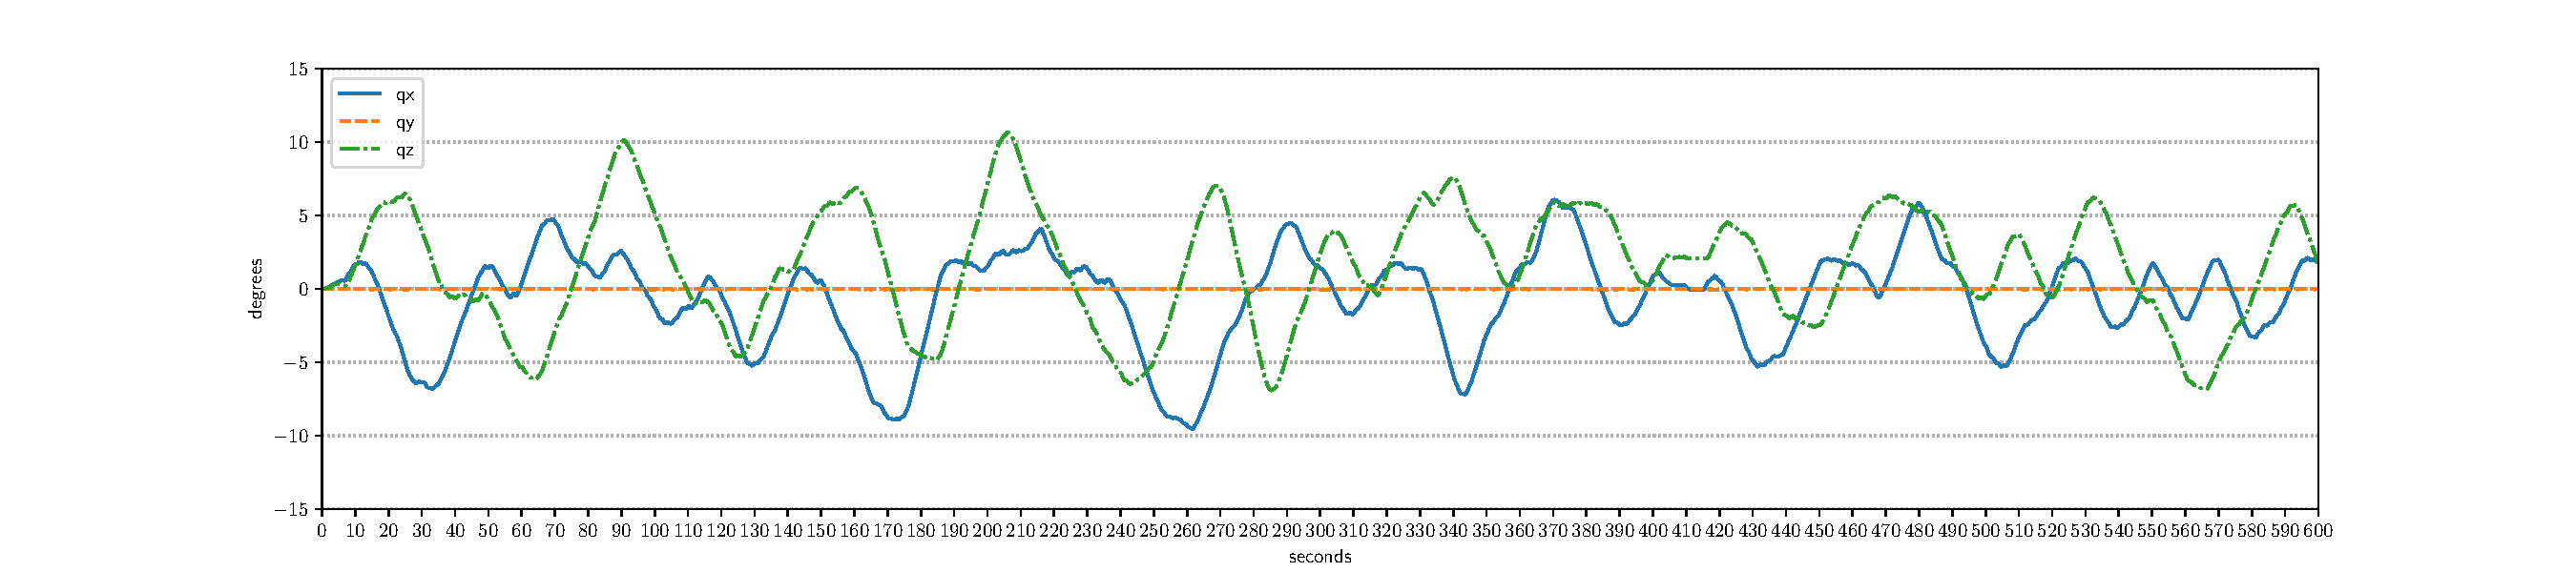
\includegraphics[width=1\textwidth, keepaspectratio]{gfx/Fig-1556-position.pdf}
		\caption{Dataset 1556}
		\label{fig:pos1}
	\end{subfigure}
	\qquad
	\begin{subfigure}[b]{1\textwidth}
		\centering
		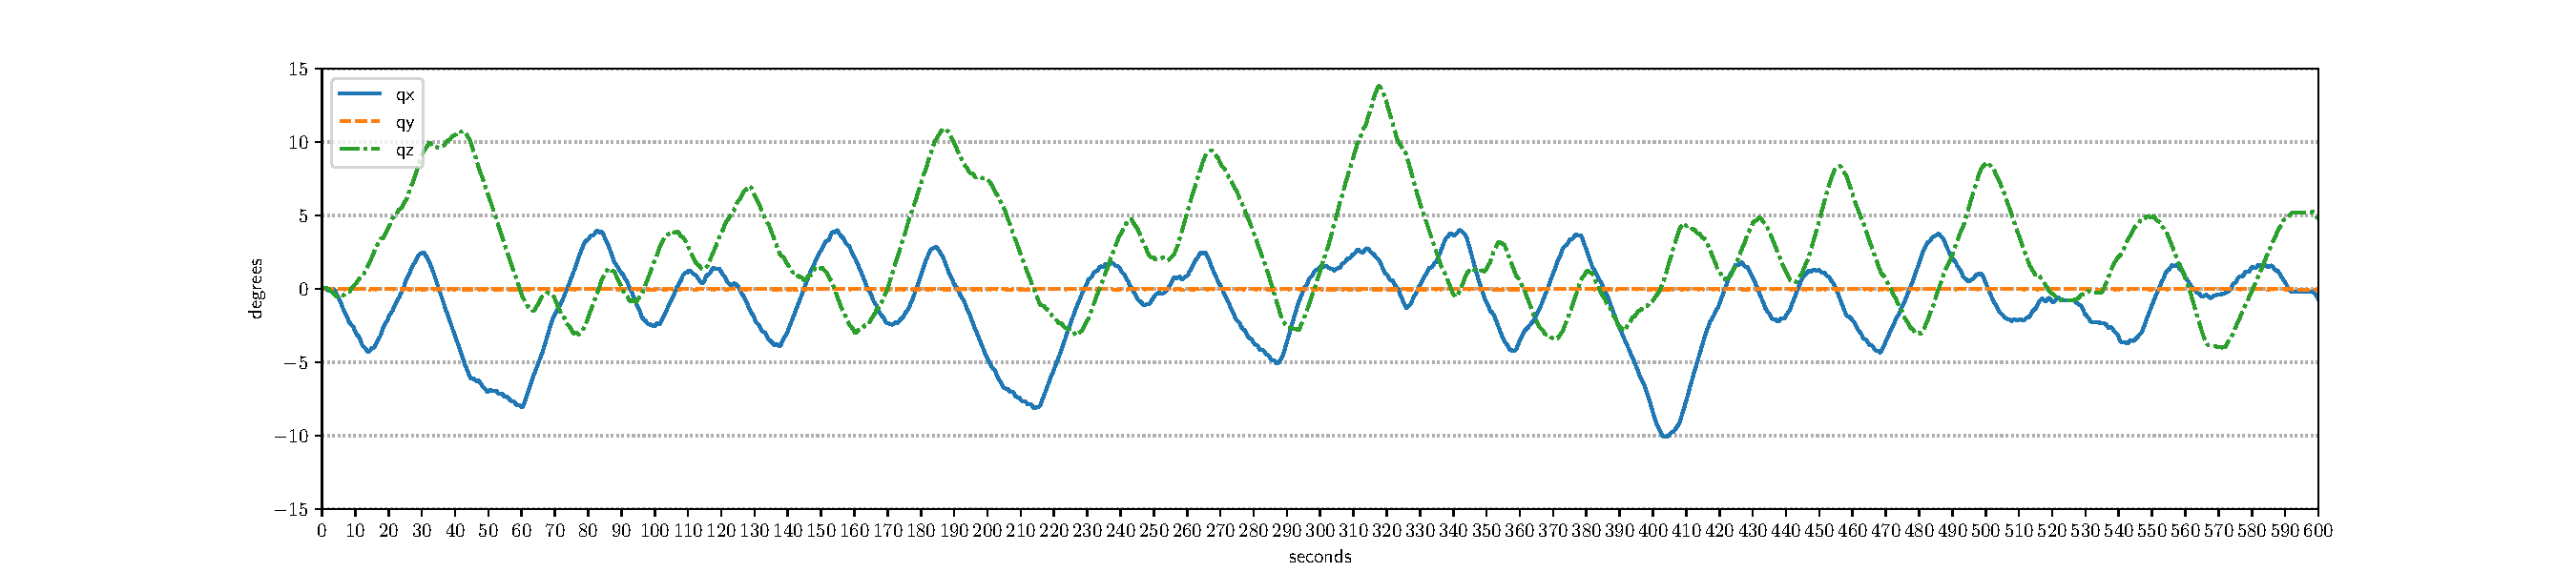
\includegraphics[width=\textwidth]{gfx/Fig-1613-position.pdf}
		\caption{Dataset 1623}
		\label{fig:pos2}
	\end{subfigure}
	\qquad
	\begin{subfigure}[b]{1\textwidth}
		\centering
		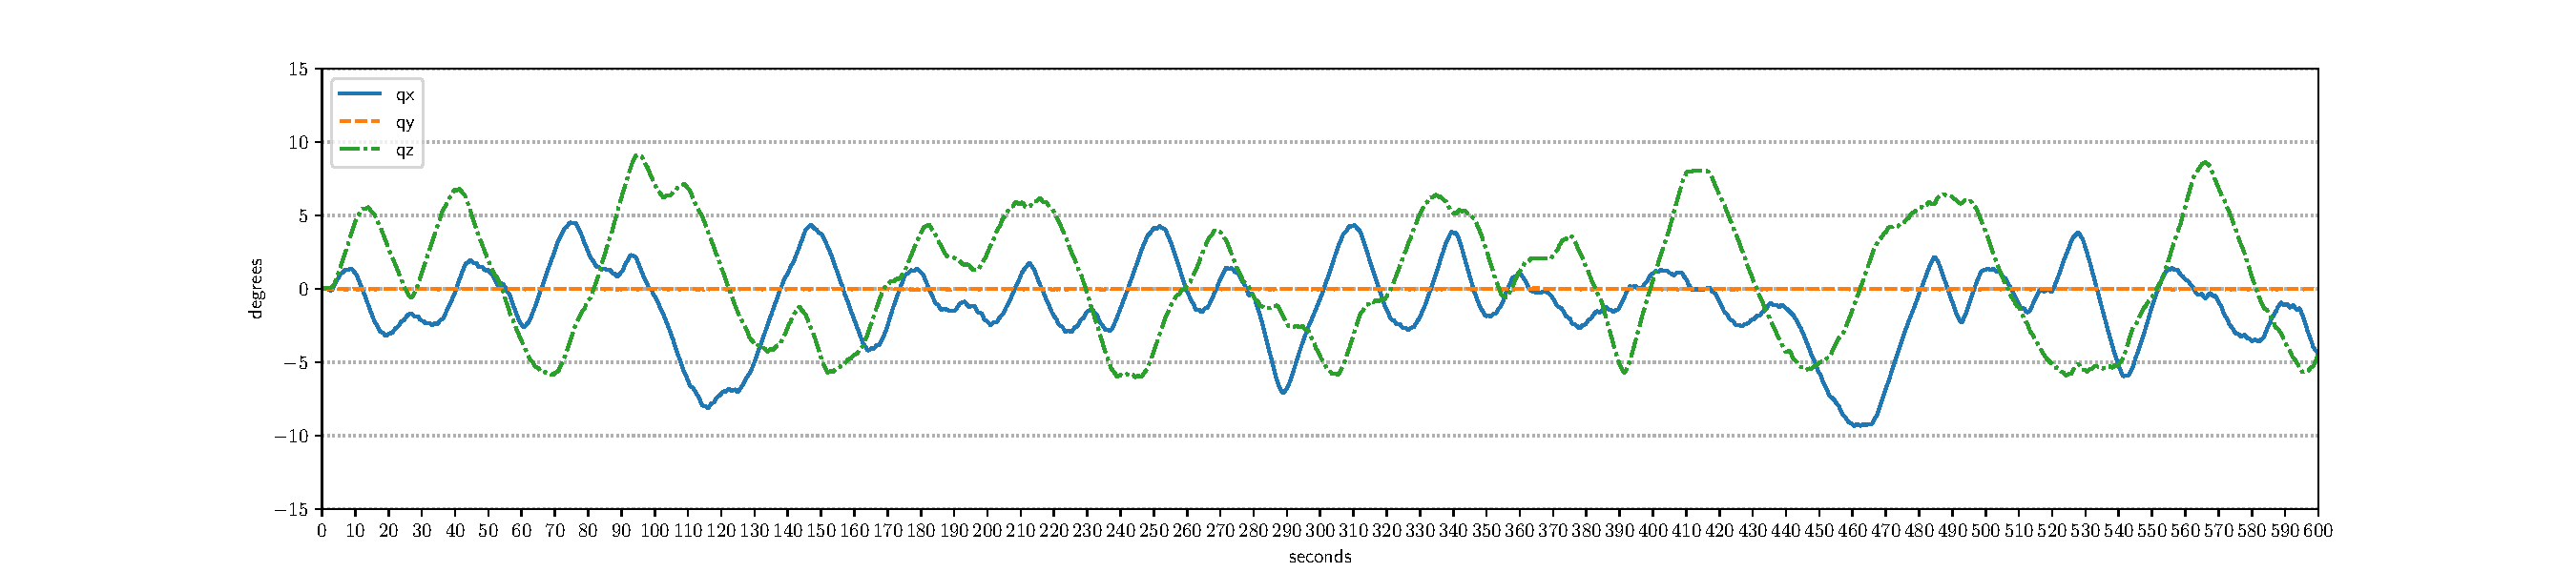
\includegraphics[width=1\textwidth, keepaspectratio]{gfx/Fig-1703-position.pdf}
		\caption{Dataset 1703}
		\label{fig:pos3}
	\end{subfigure}
	\caption{User position plots from obtained datasets (a, b, c).}
	\label{fig:datasets}
\end{figure}
First, let's start with the analysis of user position data. The figures \ref{fig:pos1}, \ref{fig:pos2}, \ref{fig:pos3} show dataset named $1556, 1623$ and $1703$ correspondingly. As a matter of fact, plotted dataset were already interpolated on the preprocessing step. Although interpolation was done before data exploration, the details about interpolation can be found in section \ref*{sec:impl:dataset:preprocessing}. The names of datasets means only a $timestamp$ in format $HH:MM$ when a dataset was obtained from HMD in laboratory space. Thus the unique name of $csv$-files on the HMD system was guaranteed for the day of experiment. In this thesis the names will be used to identify each of all three datasets. Fig. \ref{fig:datasets} shows only 3 chosen datasets from those obtained in laboratory space. All datasets indicate the same behaviour of VR users with HMD looking at the VV projected in VR space as was found out in works \cite{serhan_kalman, user_behav_volumetric}. The $MAE$ and $RMSE$ metric results tend to be similar for every dataset during training and testing.

All traces were recorded over 10 minutes long on average 12 minutes. All traces were then shortened to a precise length of 10 minutes to ensure equal data length for the purpose of visualisation and analysis. The observations based on the sample traces can be made similar as it was done by \textit{Gül et al., 2020} in their work \cite{serhan_kalman}. The user rarely moves along the y-axis. The y-axis shows the vertical movement that the users could make if they sit down or stand up. Based on the data obtained, users walked around a volumetric object in virtual reality and did not make particularly noticeable and prolonged attempts to examine the object at the lower point of the projection on a laboratory's floor since vertical movement requires more effort to crouch down and stand up. The laboratory space where the dataset was obtained was not cluttered with furniture thus users could walk around the volumetric object projected into their HMD. The figure \ref{fig:y_pos} shows an enlarged y-axis in the range from 400ms to 500ms and thus proves there is no significant change in the vertical position of the user.

\begin{figure}[htb]
	\begin{center}
		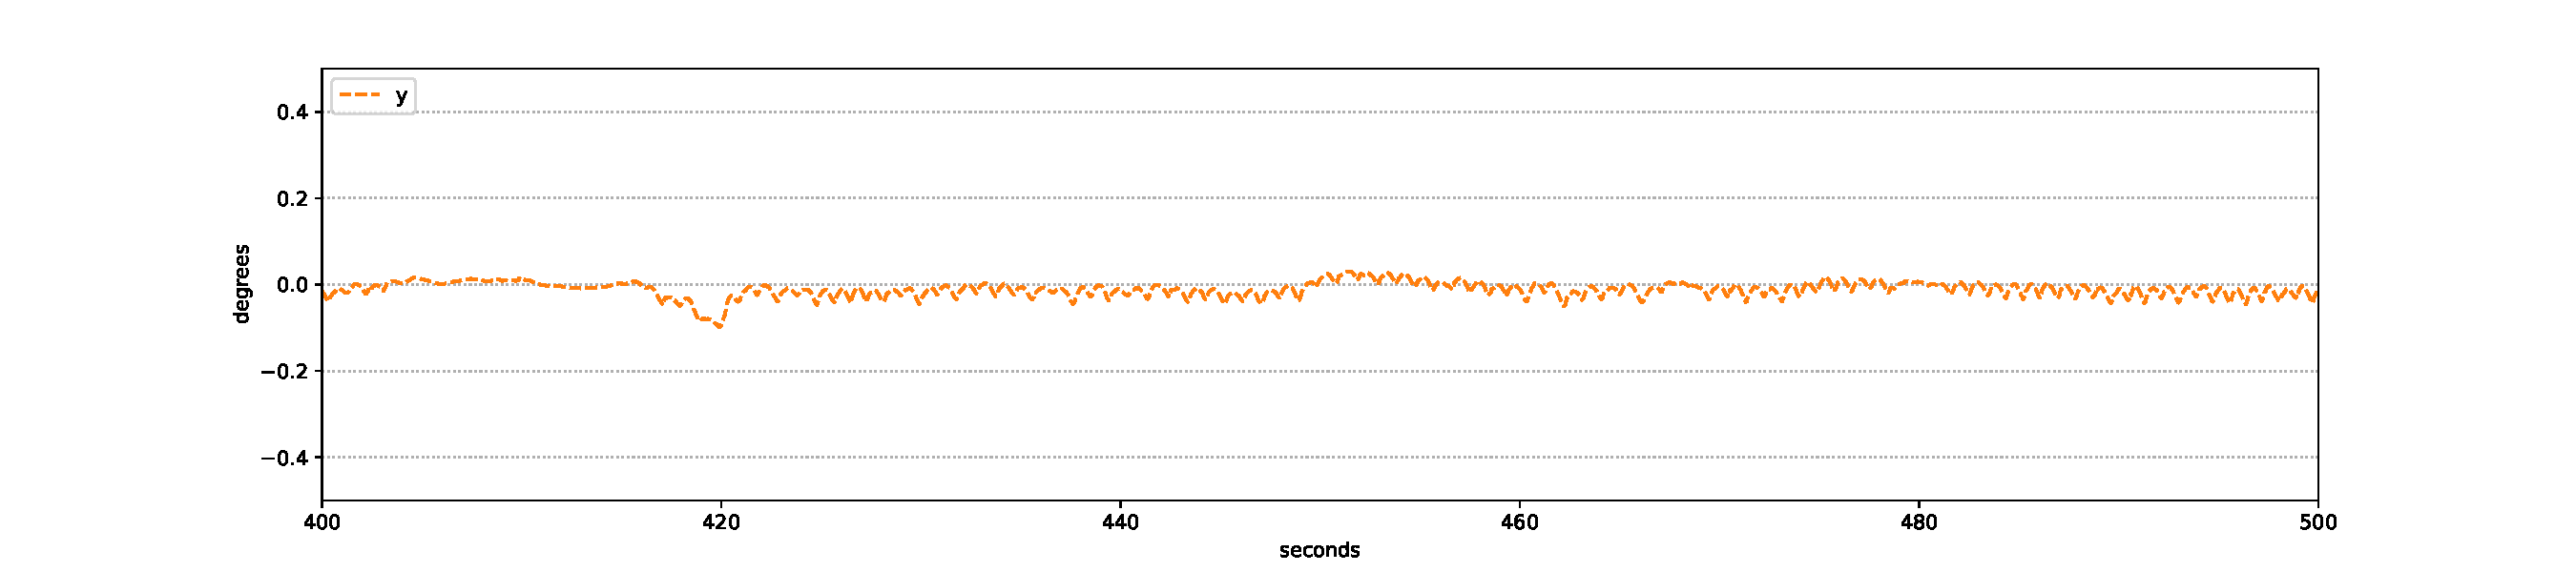
\includegraphics[width=1\textwidth, keepaspectratio]{gfx/Fig-1556-y_position.pdf}
		\caption{\label{fig:y_pos} Changes in the user's position along the Y axis in the range from 400ms to 500ms.}
	\end{center}
\end{figure}

Spatial coordinate systems on Windows (HoloLens runs on the Windows Holographic OS) must be right-handed according to the Microsoft documentation. However Unity documentation points that Unity uses a left-handed convention for its coordinate system and experiments performed in Unity with HoloLens 2 during implementation step proved that spatial coordinates in dataset recorded from left-handed system. In both kinds of coordinate systems, the positive X-axis points to the right and the positive Y-axis points up (aligned to gravity). In the recorded dataset positive Z-axis points away from a user. Spatial coordinate system of HoloLens expresses coordinate values in metres. The mean of position for axes are $X = - 0.71, Y = 0.01, Z = 1.58$ for dataset $1556$. This statistical indicator helps to judge the movement pattern in the VR environment projected inside the particular laboratory space. The user's movement along the X axis is shifted 0,7 m to the left side in the direction of the negative axis. This can be explained by the position of origin of the coordinates when the Unity application was launched. If the application was not launched strictly in the centre of the room, but rather closer to the window or wall on one side of the room, then the user had less room space from the side of the window or wall. The Y-axis shows no significant change in the movement and thus rather reflects the difference of the HMD position on the head when the user makes steps walking in the room. Mean of Y-axis of dataset $1556$ shows the average user was about 1,58 m back from the origin of the coordinate system. The VV object of a real animated human was placed 3 metres ahead of the user. It seems that users are required to step back 1-2 metres to be able to see the whole height of the placed VV object respecting the limited Field of View (FoV) of HoloLens 2. Microsoft website\footnote{https://www.microsoft.com/en-us/hololens/hardware} states the headset’s aspect ratio is 3:2, horizontal Field of View (FoV) of 43$^{\circ}$ and a vertical of 29$^{\circ}$. Indeed the standard deviation for axes $X = 3.23, Z = 3.92$ shows that the user circled the hologram (VV of a human) with an average distance 3-4 metres looking at the volumetric object from all sides. For Y-axis $Y_{std} = 0.015$ corresponds to a distance deviation from the measured mean when the user was walking in the room without significant movement up (like jumping) or down (sitting down on the floor).

%################################################

\subsection{Data preprocessing}
\label{sec:impl:dataset:preprocessing}
As was mentioned in section \ref*{sec:impl:dataset:HL}, the raw sensor data obtained from the HoloLens was unevenly sampled at 60 Hz and had different temporal distances between consecutive samples. The data preprocessing step transforms the data into a format that is more easily and effectively can be processed and visualised. Table \ref{tab:inter_data_pos} shows 20 first rows from the resulting dataset after upsampling the positional data with linear interpolation.
\begin{table}[!ht]
	\footnotesize
	\centering
	\begin{tabular}{|l|l|l|l|}
		\hline
		timestamp & x & y & z \\ [0.5ex] 
		\hline\hline
		0.0 & 0.004954389 & 0.003402365 & 0.01010712 \\ \hline
		5000000.0 & 0.0048331026667 & 0.003308667 & 0.0105062067 \\ \hline
		10000000.0 & 0.00471181633333 & 0.003214633332 & 0.01090523 \\ \hline
		15000000.0 & 0.00459053 & 0.003120769 & 0.01130438 \\ \hline
		20000000.0 & 0.004485576166 & 0.00309903333 & 0.0115486078 \\ \hline
		25000000.0 & 0.00438062233 & 0.00307733667 & 0.011792899 \\ \hline
		30000000.0 & 0.0042756685 & 0.0030556205 & 0.01203707 \\ \hline
		35000000.0 & 0.004170714667 & 0.0030339033 & 0.0122813 \\ \hline
		40000000.0 & 0.00406576084 & 0.00301218867 & 0.01252553 \\ \hline
		45000000.0 & 0.003960807 & 0.002990472 & 0.01276976 \\ \hline
		50000000.0 & 0.00390328375 & 0.00300229975 & 0.0128401975 \\ \hline
		55000000.0 & 0.0038457605 & 0.0030141275 & 0.012910635 \\ \hline
		60000000.0 & 0.00378823725 & 0.00302595525 & 0.0129810725 \\ \hline
		65000000.0 & 0.003730714 & 0.003037783 & 0.01305151 \\ \hline
		70000000.0 & 0.003651043834 & 0.00311298635 & 0.01315696 \\ \hline
		75000000.0 & 0.003571373667 & 0.00318818967 & 0.01326241 \\ \hline
		80000000.0 & 0.003491703003 & 0.003263393 & 0.01336786 \\ \hline
		85000000.0 & 0.003412033332 & 0.0033385963 & 0.01347331 \\ \hline
		90000000.0 & 0.003332363167 & 0.003413799667 & 0.01357876 \\ \hline
		95000000.0 & 0.003252693 & 0.003489003 & 0.01368421 \\ \hline
	\end{tabular}
	\caption{\label{tab:inter_data_pos}Interpolated positional data from HoloLens 2.}
\end{table}

\textit{Gül et al., 2020} obtained the similar raw dataset from the same HMD and interpolated it to obtain temporally equidistant samples. Same as it was done in work \cite{serhan_kalman}, the position and velocity data were upsampled using linear interpolation. Spherical linear interpolation was used to interpolate between rotations represented by quaternions and  table \ref{tab:inter_data_rot} lists 20 first rows from the resulting dataset after upsampling the rotational data.

\begin{table}[!ht]
	\footnotesize
	\centering
	\begin{tabular}{|l|l|l|l|}
		\hline
		qx & qy & qz  & qw \\ [0.5ex] 
		\hline\hline
		0.05225104 & -0.0092471 & -0.01470939 & 0.998482825\\ \hline
		0.052829134 & -0.0094018 & -0.01476541 & 0.9984501\\ \hline
		0.053407194	& -0.0095559 & -0.0148214108 & 0.99841708 \\ \hline
		0.053985240 & -0.00971031 & -0.0148774088 & 0.9983836 \\ \hline
		0.054563231 & -0.0098646 & -0.0149333515 & 0.99834990 \\ \hline
		0.054967034 & -0.0099280 & -0.0147404755 & 0.99832999 \\ \hline
		0.055370826 & -0.0099914 & -0.014547596 & 0.998309876 \\ \hline
		0.055774607 & -0.0100548 & -0.0143547143 & 0.998289554 \\ \hline
		0.056178376 & -0.0101182 & -0.0141618293 & 0.9982690 \\ \hline
		0.0565821344 & 0.0101816 & -0.01396894 & 0.998248298 \\ \hline
		0.0568467445 & -0.0102414 & -0.01378002 & 0.99823527 \\ \hline
		0.0567612581 & -0.01029217 & -0.01360108 & 0.998242075 \\ \hline
		0.0566757694 & -0.01034289 & -0.013422148 & 0.998248830 \\ \hline
		0.0565902782 & -0.01039361 & -0.013243212 & 0.9982555436 \\ \hline
		0.0565037268 & -0.01044992 & -0.0130706110 & 0.998262133 \\ \hline
		0.0563820024 & -0.010691806 & -0.01310865 & 0.998265955 \\ \hline
		0.0562602738 & -0.010933688 & -0.01314669 & 0.998269703 \\ \hline
		0.0561385409 & -0.011175569 & -0.013184732 & 0.9982733762 \\ \hline
		0.0560168039 & -0.011417450 & -0.013222770 & 0.99827697 \\ \hline
	\end{tabular}
	\caption{\label{tab:inter_data_rot}Interpolated rotational data from HoloLens 2.}
\end{table}

\begin{figure}[htb]
	\begin{center}
		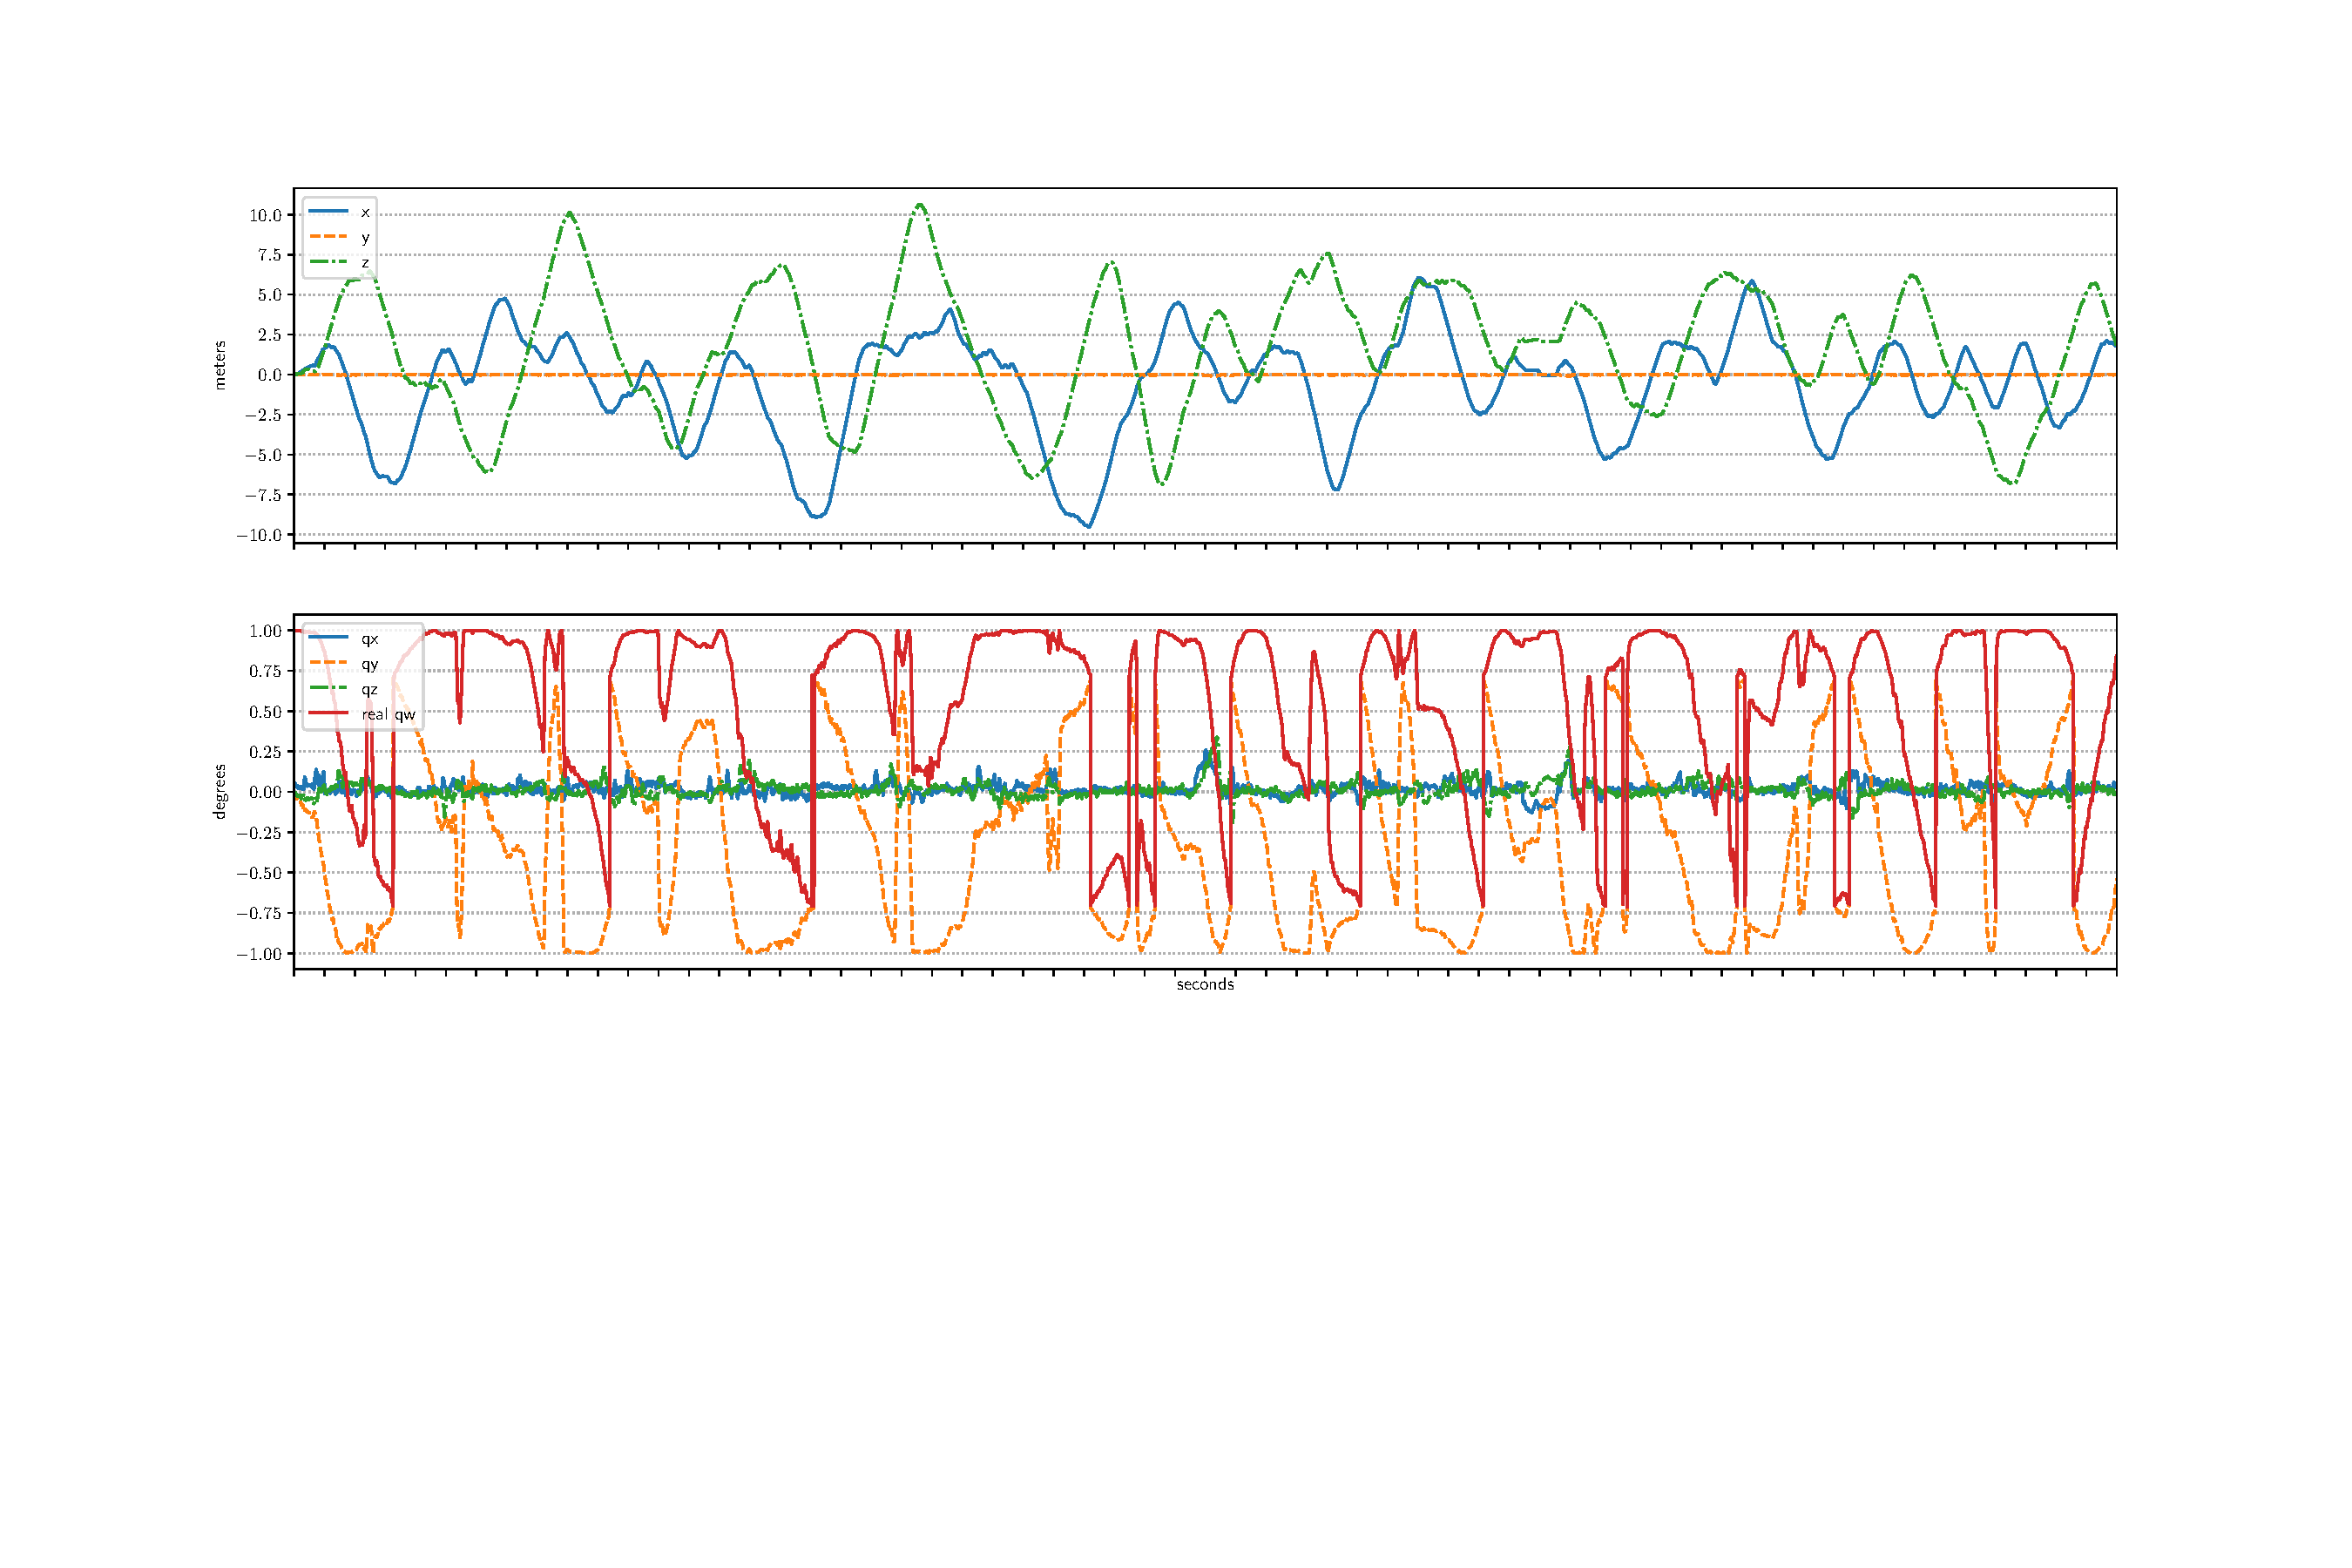
\includegraphics[width=1\textwidth, keepaspectratio]{gfx/Fig-1556-interpolated_2.pdf}
		\caption{\label{fig:inter_data}Interpolated 6-DoF dataset's user position and orientation in quaternions.}
	\end{center}
\end{figure}

After the interpolated dataset was plotted as figure \ref{fig:inter_data}, the important observations based on the sample trace could be done. While the user position data plots look appropriate for machine learning algorithms, the graph with orientation shows data that is not the perfect case for usage with machine learning technologies and could decrease the prediction rate. The real part $qw$ and the component $qy$ of quaternion have obviously discontinuous (sharp change of sign) making it hard for a predictor to learn. An orientation on quaternions is used in training, thus this data requires a few additionally preprocessing steps. Usually, when doing calculation with quaternions, quaternions must be normalised to a unit length in order to represent valid rotations \cite{principles_robot_motion_book}. During experiments with quaternions in the obtained dataset was detected that quaternion magnitudes $|| q ||$ are equal to 1. Thus the data came from a HMD already normalised, so that a quaternion in the dataset kept the orientation as it was during the user's movement with a magnitude equal to 1.0.

Next, quaternions between neighbouring points in the obtained dataset represent the very similar orientation made by the user wearing HMD step by step. The orientation plot on figure \ref{fig:norm_data} has discontinuities that can be seen on $qw$ line. As a consequence of the discontinuity (sharp change of line from negative to positive area with the same amplitude) the two neighbouring quaternions with similar rotation have significant 4D vector space between them. It makes predictions worse than what can be proved by $RMSE$ and $MAE$ rotation metrics. Flipping the sign will not affect the rotation, but it will ensure that there are no large jumps in 4D vector space when the rotation difference in rotation space (SO(3)) is small. If the negative component of quaternions is flipped into positive then the dataset, representing the same rotation without creating an artificial discontinuity in the space, will be available for model training. 

\begin{figure}[htb]
	\begin{center}
		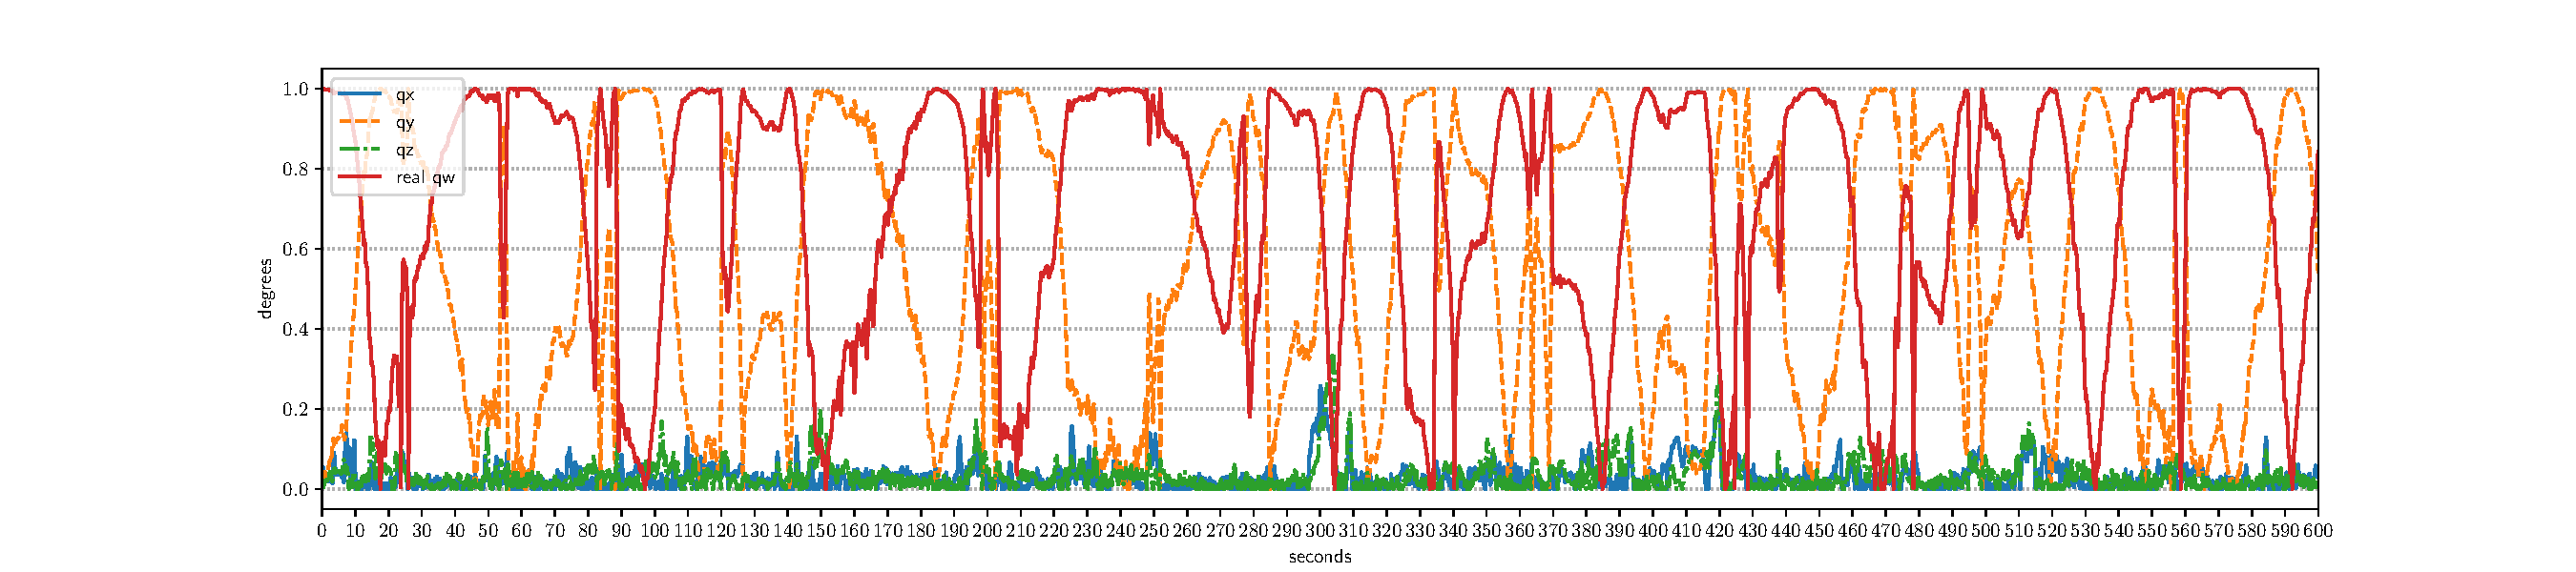
\includegraphics[width=1\textwidth, keepaspectratio]{gfx/Fig-1556-quaternions_flipped.pdf}
		\caption{\label{fig:norm_data} Quaternions from 6-DoF dataset's flipped if their real part is negative.}
	\end{center}
\end{figure}

The figure \ref{fig:compare} represents quaternions of the original interpolated dataset on the upper part of the plot and the normalised flipped quaternions on the lower part of the plot. The quaternion's components were flipped only if their real part became negative. Different from figure \ref{fig:norm_data} the limit of y-axis is set to [-1, 1] on figure \ref{fig:compare} so that the result of inverting the quaternion is easy to compare to the original data. Figure \ref{fig:compare} shows plotted data with length of 20 seconds in range 162 - 182 s from both datasets.
\begin{figure}[htb]
	\begin{center}
		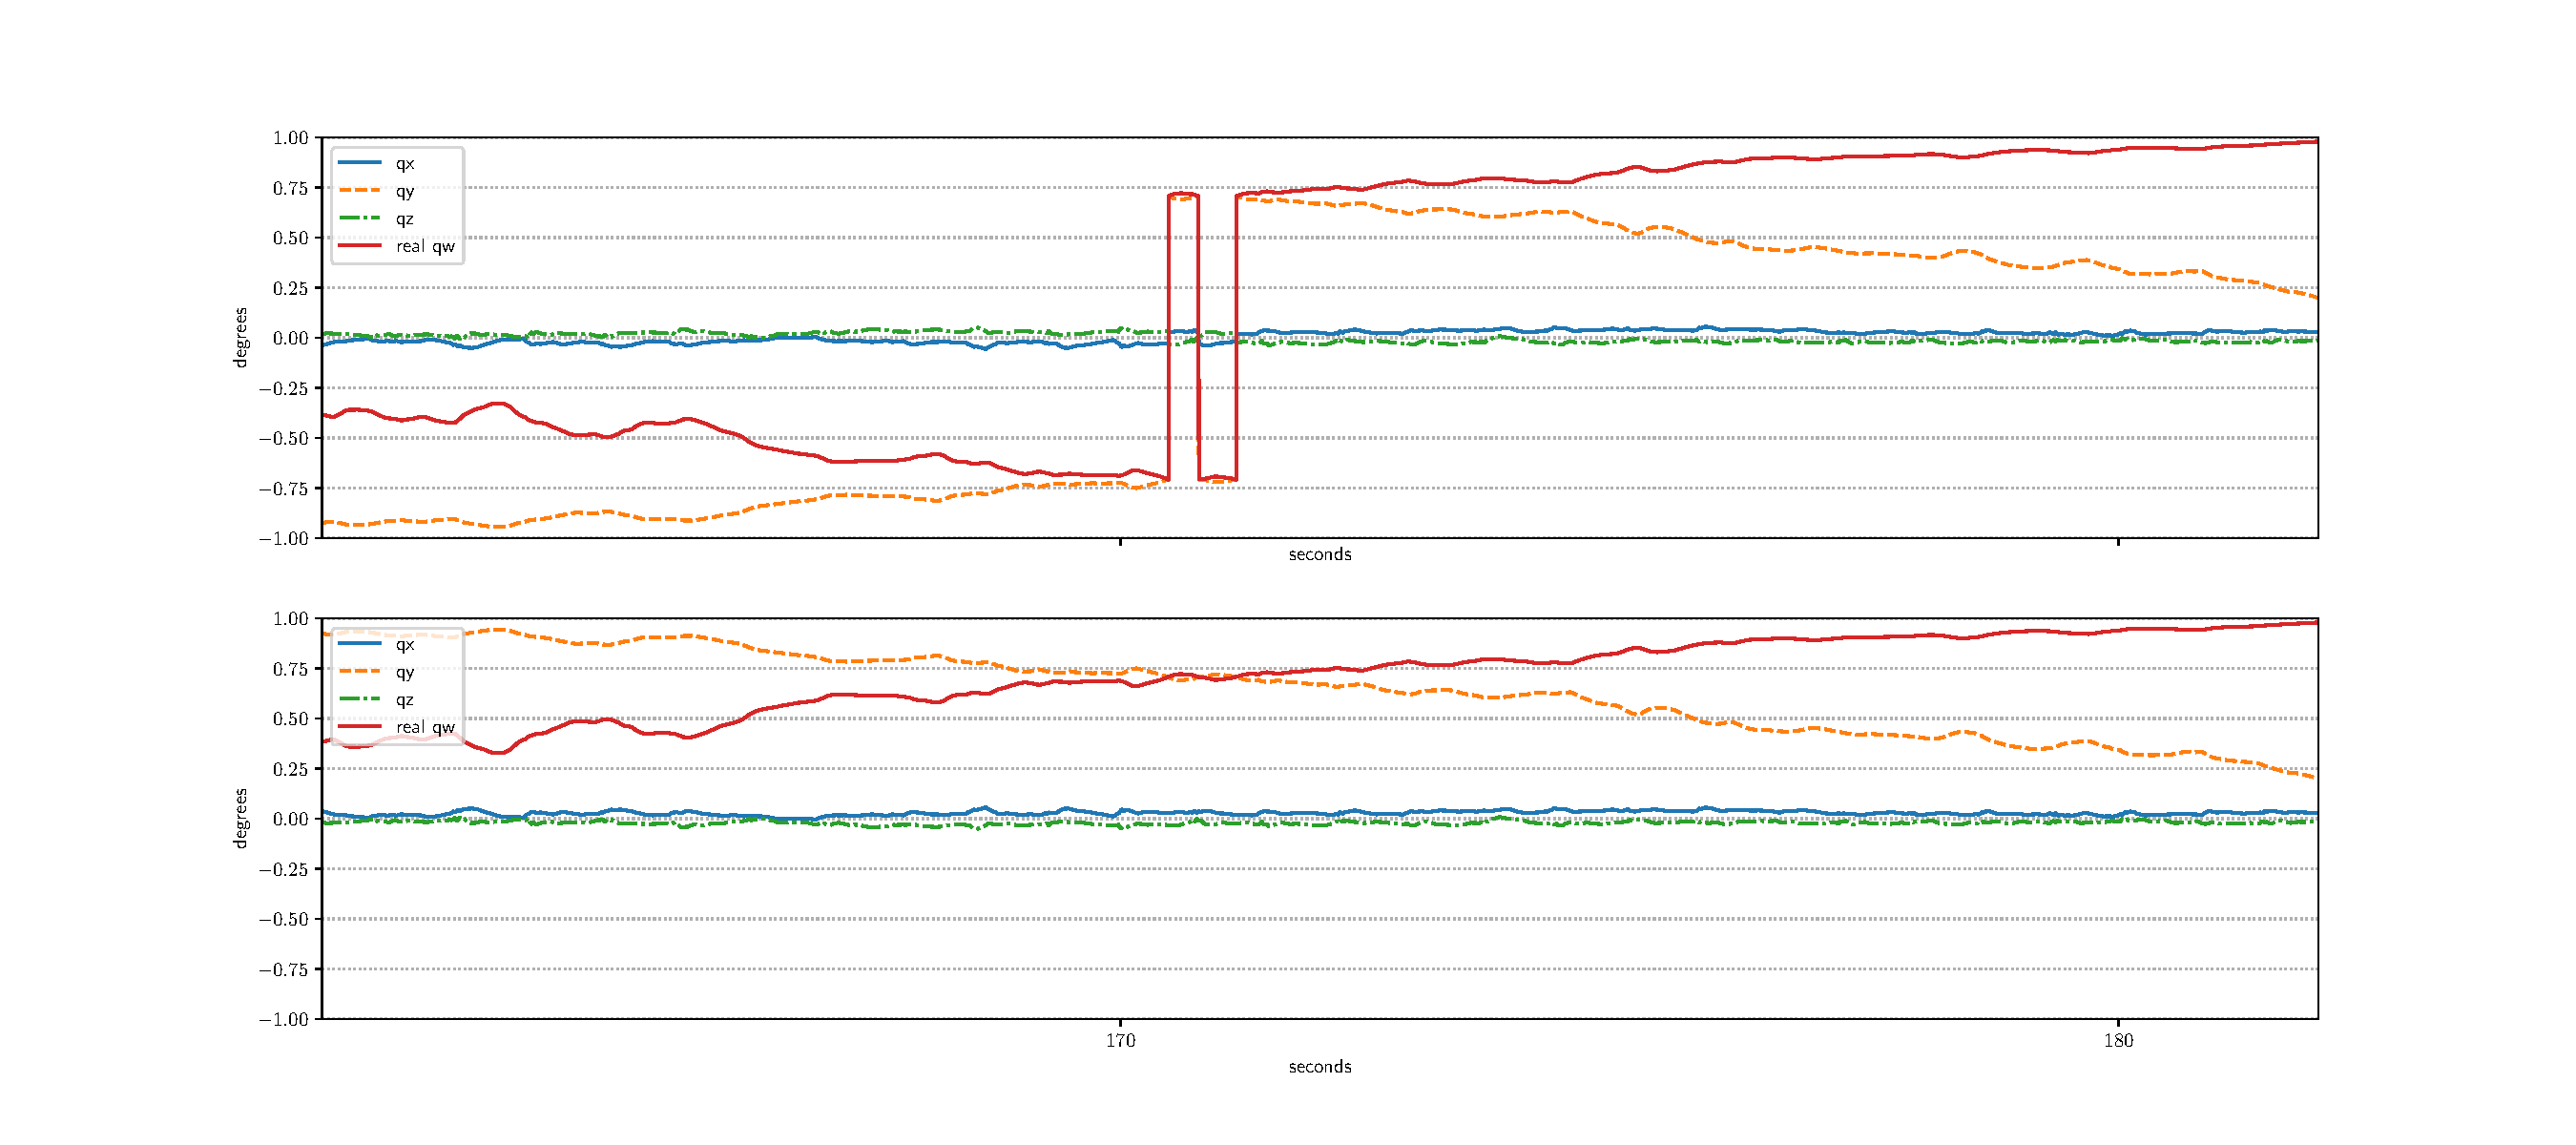
\includegraphics[width=1\textwidth, keepaspectratio]{gfx/Fig-1556-compare.pdf}
		\caption{\label{fig:compare} Enlarged quaternion plot with breaks omitted.}
	\end{center}
\end{figure}

Thus the two representations of quaternions were blended into one data set, omitting discontinuities in the time series as can be seen presented on Figure \ref{fig:norm_data}. Indeed, the $RMSE$ and $MAE$ rotation metrics were improved when the model was trained with a dataset with quaternions without sharp sign changes. More information can be found in section \ref{sec:eval:experiments}.

%''########################################

\newpage
\section{Model}
\label{sec:impl:model}
The section describes the inputs and architecture of evaluated LSTM, GRU and Bidirectional GRU models. A model itself is a mathematical representation that produces expected output based on a given input. 
\subsection{Inputs and outputs}
\label{sec:impl:model:inputs}
The correctly chosen model can discover and learn the patterns in the input dataset while being trained in order to predict new data after training. In the sections \ref{sec:impl:dataset:explor} and \ref{sec:impl:dataset:preprocessing} the obtaining and structure of 6-DoF is covered. After the data preprocessing step, the interpolated dataset with flipped negative quaternion was used for model training. The dataset itself can not be used with a model directly and a sequence data must be prepared to feed as an input into an RNN model. The 6-DoF dataset is a two-dimensional array. The first dimension of the 6-DoF dataset represents the number of timesteps of the recorded dataset. The second dimension represents the number of features of the input sequence. During data collection a 6-DoF dataset with 10 features was created. Recorded in dataset features are position $(x, y, z)$, orientation $(qx, qy, qz, qw)$ and velocity $(x, y, z)$ data. 

However PyTorch’s LSTM and GRU models expect all of their inputs to be 3D tensors. Thus 2D data must be converted into 3D data. The meaning of the axes of these tensors is important. The first axis by default is the sequence itself, the second indexes instances in the batches, and the third indexes features of the input. By specifying PyTorch's parameter $batch first = true$ the input and output tensors were provided as $(batch, seq, feature)$ instead of $(seq, batch, feature)$. This change does not apply to hidden or cell states and thus tensor containing the initial hidden for each element in the batch must be initialised as $(D * layers, batch, hidden)$. $D$ is 1 for LSTM and GRU Models and equal to 2 for their bidirectional variant. 

Usually in machine learning the dataset will be split randomly, as there’s no dependence from one observation to the other. With time series representing user position and rotation this is not a case and data have to be split with respect to time dependencies. The 6-DoF contains positional data without any seasonal characteristic and there is no obvious way to split data in groups. It is decided to split the dataset into three datasets: training, validation and test dataset. The split ratio is 60:20:20 for each corresponding dataset. Thus first 60\% of data used for training, next 20\% for validation and the rest 20\% for testing. No dimensional shuffle was applied to keep the original time dependencies. During training loop on each epoch model trained on training dataset in $train()$ mode that allows the learning process with updating of model weights. In the end each epoch model was explicitly set into evaluation mode by calling the $eval()$ function mode to turn off gradients computation and validate on the validation dataset. After the model was repeatedly trained for 500 epochs, the model then predicted new data on a never seen before test dataset.

The last step to prepare a 6-DoF dataset to be used as model input is using time steps as features. Having a historical data of user position and orientation, the next value, $X(t+n)$ must be predicted by a model from the previous n observations $Xt, X+1$, ..., and $X(t+n-1)$. Since the future values that must be predicted are already recorded in the dataset, a sliding-window approach can use prior time steps to predict the next time step and thus turn a time series dataset into a supervised learning problem. With a simple for-loop lagged observations can be created from input by shifting the values in a column by n times and removing the first n columns. The original dataset was interpolated using linear interpolation for position data and SLERP is used for quaternions. Thus, an interpolated dataset is an evenly-sampled dataset with a sampling rate of 200 Hz (5 ms). The LAT of 100 ms is used for evaluation. Thus 20 future values corresponding the $LAT = 100 ms$ must be predicted by LSTM and compared with real data to evaluate the prediction. 

Finally, the spit datasets with added sliding window were exported in standard binary $npy$-files format of NumPy. The format stores all of the shapes and the information necessary to reconstruct the array correctly even on another machine with a different architecture. Thus the spitting of the dataset is not required every time when the model trains with different hyperparameters on the GPU cluster.
 
\subsection{LSTM Model}
\label{sec:impl:model:arch:lstm}
Recurrent neural networks have recently shown promising results in many machine learning tasks, especially when input and/or output are of variable length and are coming as time series with a sequential order. Unfortunately, the known problem of RNN that was observed many years ago by e.g., \textit{Bengio et al., 1994} that it is difficult to train RNNs to capture long-term dependencies because the gradients tend to either vanish (most of the time) or explode (rarely, but with severe effects) \cite{rnn_difficults}. New approaches are needed to be implemented to reduce the negative impacts of this issue. Since traditional recurrent unit overwrites its content at each time-step, a LSTM unit is able to decide whether to keep the existing memory via the introduced gates. The Long Short-Term Memory (LSTM) has a number of minor modifications \cite{empirical_evaluation} since it was initially proposed in work \cite{lstm_orig}.
Analysis done by \textit{Qian et al., 2016} indicates that in the short term users’ head movement can be predicted with accuracy > 90\% by even using simple methods such as linear regression \cite{cellular_opt}. However in the longer term it is more difficult to achieve the good result and the average accuracy drops to about 70\% \cite{cellular_opt}. Thus LSTM model was chosen to evaluate with the 6-DoF dataset based on long term dependencies of the data. 

Since LSTM is a special kind of RNN, the RNN architecture will be briefly introduced first. RNN block consist of single computation layer with $tanh$ activation function that is used to help regulate the values flowing through the network. The tanh function squishes values to always be between -1 and 1. RNN has $h_{t}$ function of the previous cell state $h_{t-1}$ and current input$ X_{t}$. The architecture of LSTM is complexer and consists of several computational blocks that control information flow of information through the cell. The key building block behind LSTM is a structure known as $gates$. They allow LSTM to avoid the weight conflict when making decision which information from the past and current timestamp is important for correct mapping inputs to outputs. In other words, network can decide how to use gates when it is needed to keep or override the information in memory cell or access the current memory cell \cite{lstm_orig}. 

\begin{figure}[htb]
	\begin{center}
		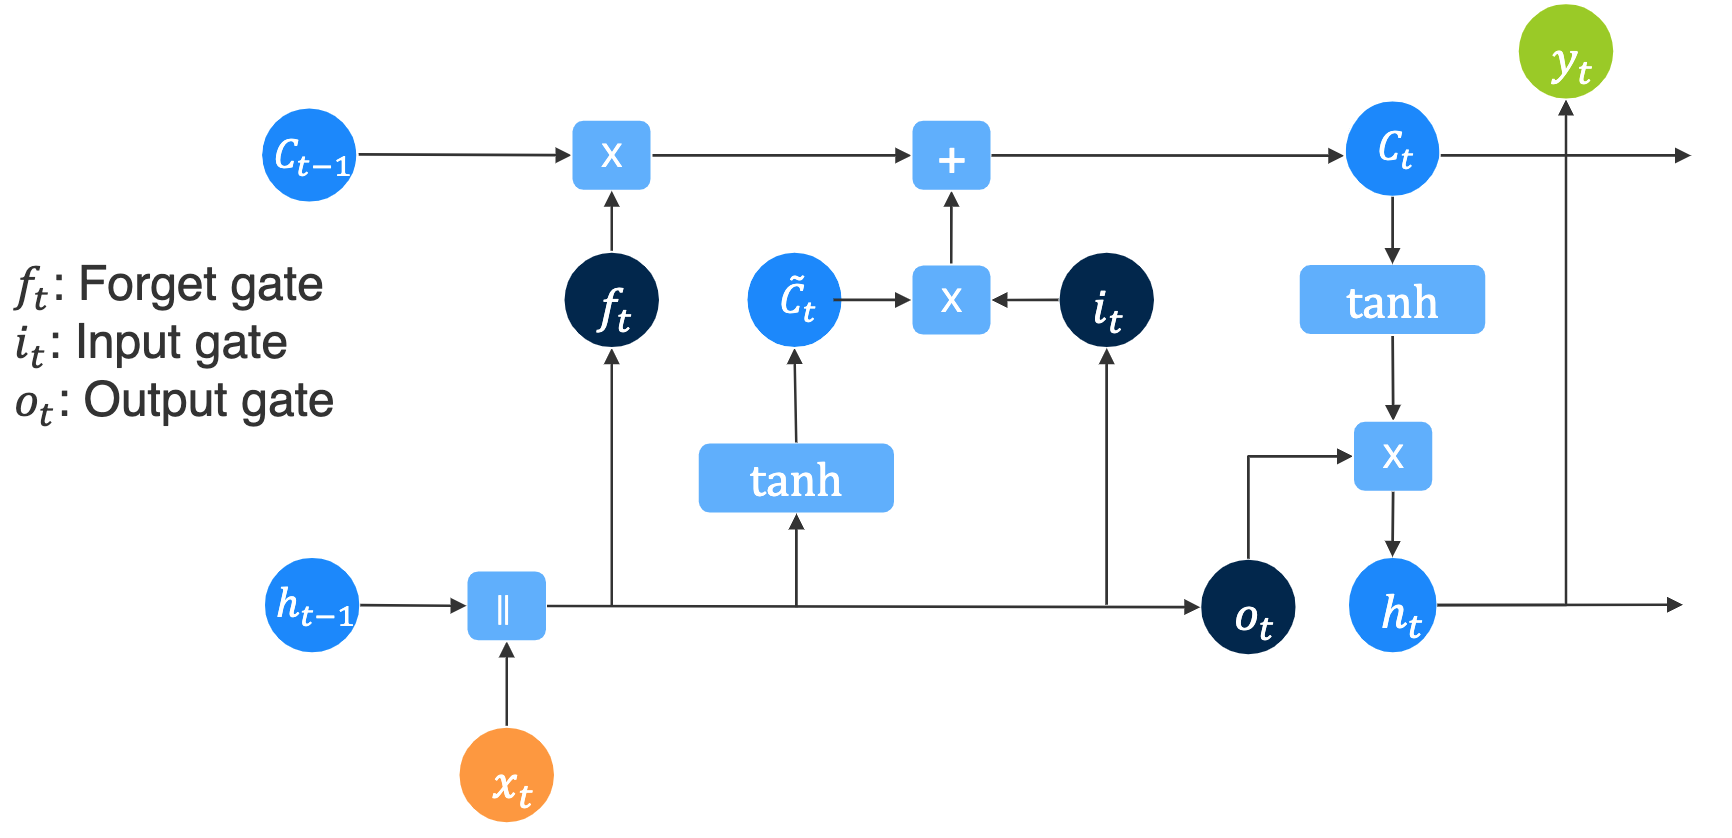
\includegraphics[width=1\textwidth, keepaspectratio]{gfx/lstm.png}
		\caption{\label{fig:lstm}Long Short-Term Memory.}
	\end{center}
\end{figure}
The LSTM architecture is illustrated\footnote{Source: Prof. Dr. Tim Landgraf, Lecture 13: Recurrent Neural Networks, WS 20/21: Machine Learning} on Fig. \ref{fig:lstm}. Using first gate $f_t$ model decides which information should be omitted from the cell in that particular time step. The sigmoid function uses the previous state (ht-1) along with the current input xt and computes the cell state using formula:
\begin{equation}
f_t = \sigma (W_{if}x_t + b_{if} + W_{hf}h_{t-1} + b_{hf})
\end{equation}
where $f_t$ is the forger gate, $h_{t}$  is the hidden state at time t, $h_{t-1}$ is the hidden state of the layer at time $t-1$ or the initial hidden state at time $0$, $\sigma$ is the sigmoid function. All LSTM gates have $sigmoid$ activations that  is similar to the $tanh$ activation but squishes values between 0 and 1. This function is useful for forgetting the information since any number getting multiplied by 0 is 0 and thus disappears from cell state. 

With $i_t$ cell state $c_t$ will be updated. First, the previous hidden state and current input are passed into a sigmoid function on input gate:
\begin{equation}
i_t = \sigma (W_{ii}x_t + b_{ii} + W_{hi}h_{t-1} + b_{hi})
\end{equation}
The transformed values between 0 and 1 meaning 0 means not important, and 1 means important will be multiplied on cell gate $\tilde{c}_t$ with the tanh output of the hidden state and current input:
\begin{equation}
\tilde{c}_t = tahn (W_{ig}x_t + b_{ig} + W_{hg}h_{t-1} + b_{hg})
\end{equation}
New cell state first gets pointwise multiplied by the forget vector anf if these values near 0 they will be dropped from the cell state. The result from the input gate is pointwise added und thus new cell state is created with values that the neural network finds relevant.
\begin{equation}
c_t = f_t \odot c_{t-1} + i_t \odot \tilde{c}_t
\end{equation}
The output gate is the last in LSTM calculations and decides what the next hidden state should be. Hidden state is also used to make a prediction because it contains information of previous inputs and thus helps to learn long term dependencies. The sigmoid function gets previous hidden state and the current input and tanh function gets the newly calculated cell state. And similar to previous step tanh output with the sigmoid output are multiplied to decide what information the hidden state should carry. The new cell state and the new hidden is then carried over to the next time step.
\begin{equation}
o_t = \sigma (W_{io}x_t + b_{io} + W_{ho}h_{t-1} + b_{ho})
\end{equation}
\begin{equation}
h_t = o_t \odot tahn(c_t)
\end{equation}

Model implementation, training loop and evaluation are done in Python using PyTorch. Model has input $[batch, sequence, features]$ with sequence equal to 20 last values what corresponds to 100 ms of historical data and 10 features that contain 3 positional, 4 rotation and 3 velocity columns. The batch size was set to $2^{7}$. The hidden dimension set experimentally after parameters grid search on GPU Cluster to be equal 512. Adam optimization algorithm is used, the maximum number of epochs was set to 500, early stopping technique (patience = 7, min. delta = 0,05) was used to avoid overfitting. Additionally, the learning rate was decreased by 50\% from initial value of 0.0001 every 30 epochs. The learning rate is a parameter that determines how much an updating step influences the current value of the weights. Adjustable learning rate was proposed in works \cite{delay_compensation_360, telepresence} and implementing this option had improved prediction and allowed model to learn patterns correctly without overfitting. Weight decay of Adam optimiser experimentally is set to a small value of $1e-12$ . Thus this additional term in the weight update rule less causes the weights to exponentially decay to zero, large weights were less penalizes and model could successfully learn the long term dependencies and thus constantly decrease both training loss and validation loss  and stabilize them at a specific point. 

The high performance was achieved event without additional activation functions with simple one-layered architecture represented below:
\begin{lstlisting}[caption={One-layered LSTM with sliding window},captionpos=b]
LSTMModel1(
(lstm): LSTM(10, 512, batch_first=True)
(fc): Linear(in_features=512, out_features=7, bias=True)
==================================================================
Layer (type:depth-idx)          Output Shape         Param #
==================================================================
LSTMModel1                       [128, 20, 7]              --
	--- LSTM: 1-1            [128, 20, 512]     1,073,152
	--- Linear: 1-2          [128, 20, 7]           3,591
==================================================================
Total params: 1,076,743
Trainable params: 1,076,743
Non-trainable params: 0
==================================================================
\end{lstlisting}

Since only position and rotation data of similar range is used in 6-DoF dataset, no scaler for the features is applied.  Experiments showed that normalization of values between [0..1] and between [-1..1] results to higher MSE and RMSE. Already preprocessed interpolated datasets with flipped negative quaternions is loaded in with respect to sequential order as training, validation and test dataset from $npy$-files. Additional extended LSTM architectures were implemented and tried with HoloLens 2 6-DoF dataset. For example, the non-linear activation functions $ReLU$ and $Mish$ were tried in order to get more sensitivity to the activation sum input and avoid easy saturation. Thus the nodes in model should be only deactivated if the output of is less than 0. Model variant with $ReLU$ experimentally resulted to produce higher MAE and RMSE compared to LSTM1 and therefore was rejected for a final deployment. Since LSTM2 Model has the similar architecture as following afterwards LSTM3, it is not listed separately 

LSTM3 uses a new activation function $Mish$ that was presented in machine learning scene in 2019 in work \cite{mish} and is a self-regularized non-monotonic activation function which can be mathematically defined as $f(x)=xtanh(softplus(x))$. Mish is a smooth, continuous activation function and allows to have better gradient flow compared to ReLU that tends to have a lot of sharp transitions \cite{mish}. The LSTM3 model improved MAE and RMSE mertics. Model's batch size changed to $2^{10}$. Additional linear layer with additional $Mish$-function is added in order to double the hidden size of LSTM. Weight decay of Adam optimiser is experimentally set to $3e-14$ with LSTM3 model.
 
\begin{lstlisting}[caption={LSTM3 with Mish activation function},captionpos=b]
LSTMModel3(
(lstm): LSTM(10, 512, batch_first=True)
(mish_1): Mish()
(fc_1): Linear(in_features=512, out_features=1024, bias=True)
(mish_2): Mish()
(fc_2): Linear(in_features=1024, out_features=7, bias=True)

==================================================================
Layer (type:depth-idx)                   Output Shape              Param #
==================================================================
LSTMModel2                   [1024, 20, 7]              --
	--- LSTM: 1-1        [1024, 20, 512]            1,073,152
	--- Mish: 1-2        [1024, 20, 512]            --
	--- Linear: 1-3      [1024, 20, 1024]           525,312
	--- Mish: 1-4        [1024, 20, 1024]           --
	--- Linear: 1-5      [1024, 20, 7]              7,175
==================================================================
Total params: 1,605,639
Trainable params: 1,605,639
Non-trainable params: 0
==================================================================
\end{lstlisting}

LSTM4 Model is a three-layered stacked LSTM with introduced additional dropout  added after all but last recurrent layer and Mish activation function. This design decision is made in order to try whether adding more components to the neural network could mean the improvement upon simpler model on 6-DoF dataset. By adding more LSTM layers the model parameters that have to be trained were increased in 5 times from 1,605,639 to 7,901,191 trainable parameters. When the model parameters are getting large in count, the model gets more complex, having hard time fitting on the training instances as it needs to optimize parameters in a way that can optimally fit the training instances. The time need for training increased noticeable even on GPU Cluster. Finally, LSTM4 resulted in significant higher MAE and RMSE metrics and thus this architecture is rejected.  

This models LSTM1 and LSTM3 are considered to be the best evaluated LSTM models that can predict the future data based on past 20 values (100 ms) in 6-DoF VR environment using sensor data from HMD for LAT of 100 ms. Although sufficient results for prediction and low MAE and RMSE metrics are already obtained with LSTM model, the GRU and bidirectional models will be implemented in order to evaluate their performance and potentially to find the better model architecture. 

\subsection{GRU Model}
\label{sec:impl:model:arch:gru}
Another approach called a gated recurrent unit (GRU) can adaptively capture dependencies of different time scales without having a separate memory cells \cite{empirical_evaluation}. It is similar to an LSTM, but only has two gates - a reset gate and an update gate. Although architecture does not provide an output gate, with fewer parameters it can generally easier and faster be trained than LSTM.  GRU Model can catch the long-term dependencies in the data obtained from HMD that are otherwise are hidden by the effect of short-term dependencies from the standard RNN models. This chapter decribes GRU model that implemented to predict future values with 6-DoF dataset obtained from HoloLens 2. \\

\begin{figure}[htb]
	\begin{center}
		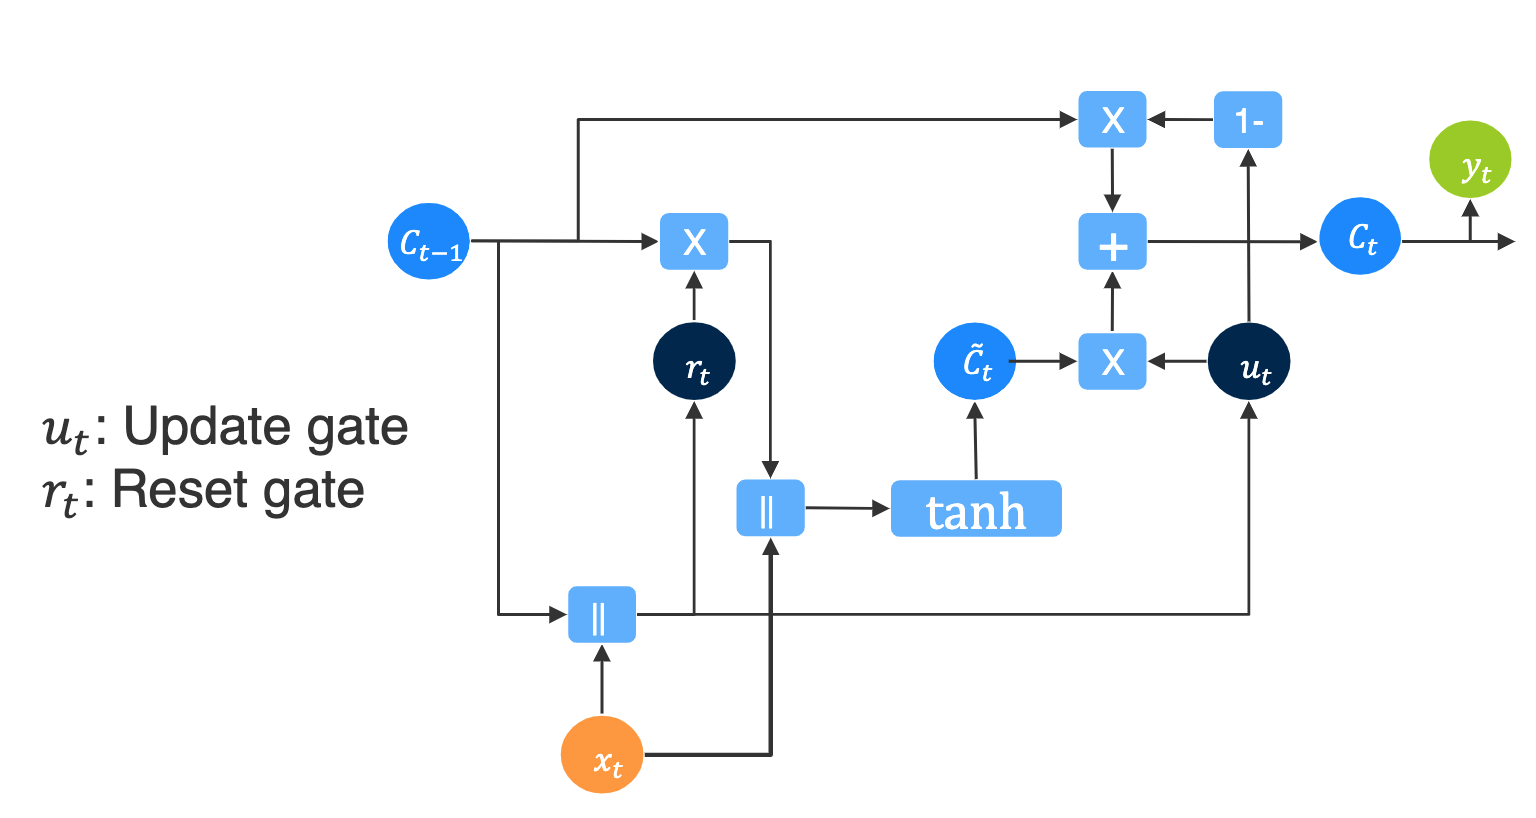
\includegraphics[width=1\textwidth, keepaspectratio]{gfx/gru.png}
		\caption{\label{fig:gru}Gated Recurrent Unit.}
	\end{center}
\end{figure}

The GRU architecture is illustrated\footnote{Source: Prof. Dr. Tim Landgraf, Lecture 13: Recurrent Neural Networks, WS 20/21: Machine Learning} on Fig. \ref{fig:gru}. GRU avoids the vanishing gradient problem of a standard RNN with only two gates that decide what information should be passed to the final output. The update gate plugs $x_t$ into the network unit and multiplied with its own weight $W_{iz}$. The same multiplication is done with previous hidden state $h_(t-1)$ that has its own weight $W_{hz}$. Both results are added together and a sigmoid activation function is applied to squash the result between 0 and 1. The mathematical expression of this calculation is as following:
\begin{equation}
z_t = \sigma (W_{iz}x_t + b_{iz} + W_{hz}h_{t-1} + b_{hz})
\end{equation}
where  $z_t$ is an update gate, $h_{t}$  is the hidden state at time t, $h_{t-1}$ is the hidden state of the layer at time $t-1$ or the initial hidden state at time $0$, $\sigma$ is the sigmoid function. With these matrix multiplications model can determine how much of the past information from previous time steps needs to be passed to the next to predict future values. 

The reset gates does what its name means - gate can reset the state of the model and thus model decides how much of the past information to forget. It is an useful option when context changes in the historical data and previous values are not more relevant to produce future values. With powerful update gate the model can decide to copy all the information from the past and eliminate the risk of vanishing gradient. The formula of the reset gate is:
\begin{equation}
r_t = \sigma (W_{ir}x_t + b_{ir} + W_{hr}h_{t-1} + b_{hr})
\end{equation}
Both gates will affect the final output. A new memory content will use the reset gate to store the relevant information from the past. It is calculated as follows:
\begin{equation}
n_t = tahn (W_{in}x_t + b_{in} + r_t * W_{hn}h_{t-1} + b_{hn})
\end{equation}
As the last step, the network calculates vector which holds information for the current unit and passes $h_t$ to the network. The formula shows that update gates is used to determine what information from previous steps will be passed into the memory. Additionally, calculated recently new memory gate $n_t$ controls the amount from current data to be added into long memory.  That is done as follows:
\begin{equation}
h_t = (1 - z_t) * n_t + z_t * h_{t-1}
\end{equation}

GRU model implementation, training loop and evaluation are done similar to LSTM in Python using PyTorch. Model has same input $[batch, sequence, features]$ with sequence equal to 20 last values and 10 features (3 positional, 4 rotation and 3 velocity columns). The batch size was increased to $2^{9}$. The hidden dimension  is 512 nodes. Same as with LSTM, Adam optimization, the extended version of stochastic gradient descent and nowadays common algorithm for ML tasks, used for GRU Model.  Adjustable learning rate is modified to decrease by 60\% from initial value of 0.0001 every 50 epochs. Weight decay kept the same value of $1e-12$ . 

The maximum number of epochs was set to 500, early stopping technique with same patience and delta as in LSTM was used to avoid overfitting. Model requires less epochs to learn and can predict better than LSTM. Although the error decreases very slowly after 150-200 epochs, the model converged to a smallest achievable error after 500 epochs. The model is overtrained with 1000 epochs if trained without early stopping technique.

Different to LSTM Model, the best performance was achieved with pure GRU model without additional activation functions with simple one-layered architecture represented below:
\begin{lstlisting}[caption={GRU1 with Sliding Window},captionpos=b]
GRUModel1(
(gru): GRU(10, 512, batch_first=True)
(fc): Linear(in_features=512, out_features=7, bias=True)
)
==================================================================
Layer (type:depth-idx)                   Output Shape              Param #
==================================================================
GRUModel1                    [512, 20, 7]             --
	--- GRU: 1-1         [512, 20, 1024]            804,864
	--- Linear: 1-2      [512, 20, 7]              3,591
=================================================================
Total params: 808,455
Trainable params: 808,455
Non-trainable params: 0
=================================================================
\end{lstlisting}

From listing above is clear, that pure GRU1 has 25\% less trainable parameters as pure LSTM1 and twice less trainable parameters as LSTM3 that uses additional activation and linear functions. Moreover the result of prediction of future values are preciser than those obtained with LSTM1 and LSTM3 and has significant smaller the MAE and RMSE metrics (more information about results of prediction with LSTM and GRU models can be found in chapter \ref{sec:eval:experiments:lstm} and \ref{sec:eval:experiments:gru}). 

Additionally to GRU1 several different architectures were implemented and tested. The GRU2 model has $ReLU$-activation function and GRU3 has $Mish$-activation function. Similar to LSTM, using of $ReLU$ did not improved the predictions. Different to LSTM, using of $Mish$ also worsened the results.     

Different quite similar architectures using $Mish$ activation function were implemented and tested with parameters grid search on GPU Cluster. GRU31 using only one $Mish$ activation compared to LSTM3 and GRU3 with two activation layer accompanied with linear layers. GRU32 and GRU35 use additionally dropout layer(s) with different parameters and combinations with linear layer(s). In GRU33 adaptive max pooling over an input signal is done to in part to help over-fitting by providing an abstracted form of the representation. Both models performed worse then those one without dropout techniques even though it was tried to train the model longer for 1000 or 2000 epochs. Every architecture including GRU1 was also tried as 3-layered and 8-layered stacked GRU and all results similar to stacked LSTM were significant worse and took noticeable more computational time as 1-layered variants.

Thus model GRU1 is considered as best evaluated model that predicts accurately the future values for LAT of 100 ms based on past 20 values (100 ms) in 6-DoF VR environment using sensor data from HMD.

\subsection{Bidirectional GRU Model}
\label{sec:impl:model:arch:bi-gru}

The last RNN variant evaluated in this master thesis is a bidirectional GRU model. From related works is known that despite the complex architecture and more historical data available for analysis and training, the prediction results do not exceed the results of a simple model. This section aims the goal to check whether the results of prediction on 6-DoF dataset are similat to those from related works.

A typical state in an RNN (simple RNN, GRU, or LSTM) relies on the past and the present events. A state at time $t$ depends on the states $x_1, x_2,..., x_{t-1}, x_t$. However, there can be situations where a prediction depends on the past, present, and future events. Theoretically if the future information will be available during the prediction, it can increase the prediction accuracy. For example, predicting a user position in the future to be included in a sequence of movements might require us to look into the future, i.e., particular future position at time $t$ could depend on a future event like turning right, left, accelerating or stopping. Bidirectional RNNs enables straight (past) and reverse traversal of input (future). Computationally Bi-RNNs are a combination of two simple RNNs for moving data beginning from the start of the data sequence, and parallel to that a backward moving occurs beginning from the end of the data sequence. Based on the type of used RNN blocks, Bi-RNN can either be simple RNNs, GRUs, or LSTMs. This section describes the usage if Bi-GRU Model because the best results were achieved with GRU1 Model and therefore no Bi-LSTM implementation was undertaken.

A Bi-GRU has an additional hidden layer to accommodate the backward training process. At any given time 
$t$, the forward and backward hidden states are updated as follows:
\begin{equation}
A_t(Forward) = \sigma (W_{xa}^{forward}x_t + b_{a}^{forward} + W_{aa}^{forward}A_{t-1})
\end{equation}
\begin{equation}
A_t(Backward) = \sigma (W_{xa}^{backward}x_t + b_{a}^{backward} + W_{aa}^{backward}A_{t+1})
\end{equation}
where 
$\sigma$ is the activation function, W is the weight matrix, and b is the bias. The hidden state at time $t$ is given by a combination of $A_t(Forward)$ and $A_t(Backward)$. The output at any given hidden state is:
\begin{equation}
O_t = H_t * W_{ay} + b_y
\end{equation}
During the training of Bi-GRU forward and backward passes happening simultaneously and thus updating the weights for the two processes could happen at the same point of time. If standard RNN Backpropagation Through Time algorithm would be applied to Bi-RNN, it could lead to erroneous results. Thus, modified algorithm is used for training a Bi-RNN to accommodate forward and backward passes separately. Thereby both the forward and backward passes together train bidirectional model. 

Model implementation done similar to GRU in Python with PyTorch. When parameter $bidirectional=True$ is specified in $nn.GRU$, PyTorch takes care about correctness of forward and backward passes and combines two GRU model by doubling the hidden dimension size. The output will be $(batch, seqeunce, hidden_size * 2)$ where the $hidden_size * 2$ features are the forward features concatenated with the backward features. The model is listed below: 
\begin{lstlisting}[caption={Bidirectional GRU Model},captionpos=b]
GRUModelBiDir1(
(init_linear): Linear(in_features=10, out_features=10, bias=True)
(bi_gru): GRU(10, 512, batch_first=True, bidirectional=True)
(out_linear): Linear(in_features=1024, out_features=7, bias=True)
)
===============================================================
Layer (type:depth-idx)                   Output Shape              Param #
===============================================================
GRUModelBiDir1                   [512, 20, 7]              --
	--- Linear: 1-1          [512, 20, 10]             110
	--- GRU: 1-2             [512, 20, 1024]           1,609,728
	--- Linear: 1-3          [512, 20, 7]              7,175
===============================================================
Total params: 1,617,013
Trainable params: 1,617,013
Non-trainable params: 0
\end{lstlisting}

The interesting thing that PyTorch requires the initialisation of $h_0$ initial state to use doubled amount of layer dimension. This one layered GRU will be initialized in PyTorch as 2-layered. It was already proved by experiments on GPU Cluster that any combinations of stacked RNN Models leads to lower prediction accuracy. Anyway it is worth to evaluate whether the accommodated separately forward and backward passes could improve the model performance.  
\begin{lstlisting}[caption={Bidirectional GRU h0 Layer},captionpos=b]
# Initializing hidden state for first input with zeros
h0 = torch.zeros(self.layer_dim * 2, x.size(0), self.hidden_dim).requires_grad_()
\end{lstlisting}

Listing above shows GRUModelBiDir1 that was implemented and evaluated additionally with GRUModelBiDir2 model with $Mish$ activation function. Same as in work of \textit{Chang et al., 2020}, the Bi-GRU performs the worst among all models. The details of evaluation can be found the section \ref{sec:eval:experiments:bi-gru}.

%''######################################

\subsection{Development}
\label{sec:impl:model:dev}
This section presents as well the development of the Unity application for obtaining the dataset, as the training loop in PyTorch used for all models and shortly describes a process of developing a GPU application. 

\subsubsection{Unity application}
\label{sec:impl:model:dev:unity}
An application was developed in Unity with the Mixed Reality Toolkit (MRTK) and deployed on HoloLens 2. The goal of the application is to obtain the user position and orientation during the time when a user wears a HMD. MRTK provides a cross-platform input system, components, and common building blocks for spatial interactions. The Unity Application was finally built using Visual Studio and deployed using Wi-Fi connection. To enable the deployment on HoloLens 2, Windows 10 has Developer Mode to be turned on and HoloLens must be paired with a Visual Studio using a PIN displayed on HoloLens. Later in final App version, that was used for data collection, the volumetric animated object was added in scene. It consist of 359 frames each with its own mesh. It drastically increased the size of Unity App and the deployment using USB was used instead of Wi-Fi connection.

In Unity, the Main Camera is always the primary stereo rendering component attached to HMD and it is rendering everything the user sees \footnote{https://docs.microsoft.com/en-us/windows/mixed-reality/develop/unity/camera-in-unity}. The starting position of the user is set to $(0, 0, 0)$ during the application launch and the Main Camera tracks movement of the user's head. Although HoloLens allows to build a world-scale application, the room-scale experience was selected for spatial coordinate system. This lets users to walk around within the 10-meter boundary what is quite enough for user's movements inside the laboratory space and simultaneously watching the volumetric video object. Fig. \ref{fig:josh} illustrates implemented Unity 3D Application window with placed obj-animation, underlying code and scene.

\begin{figure}[htb]
	\begin{center}
		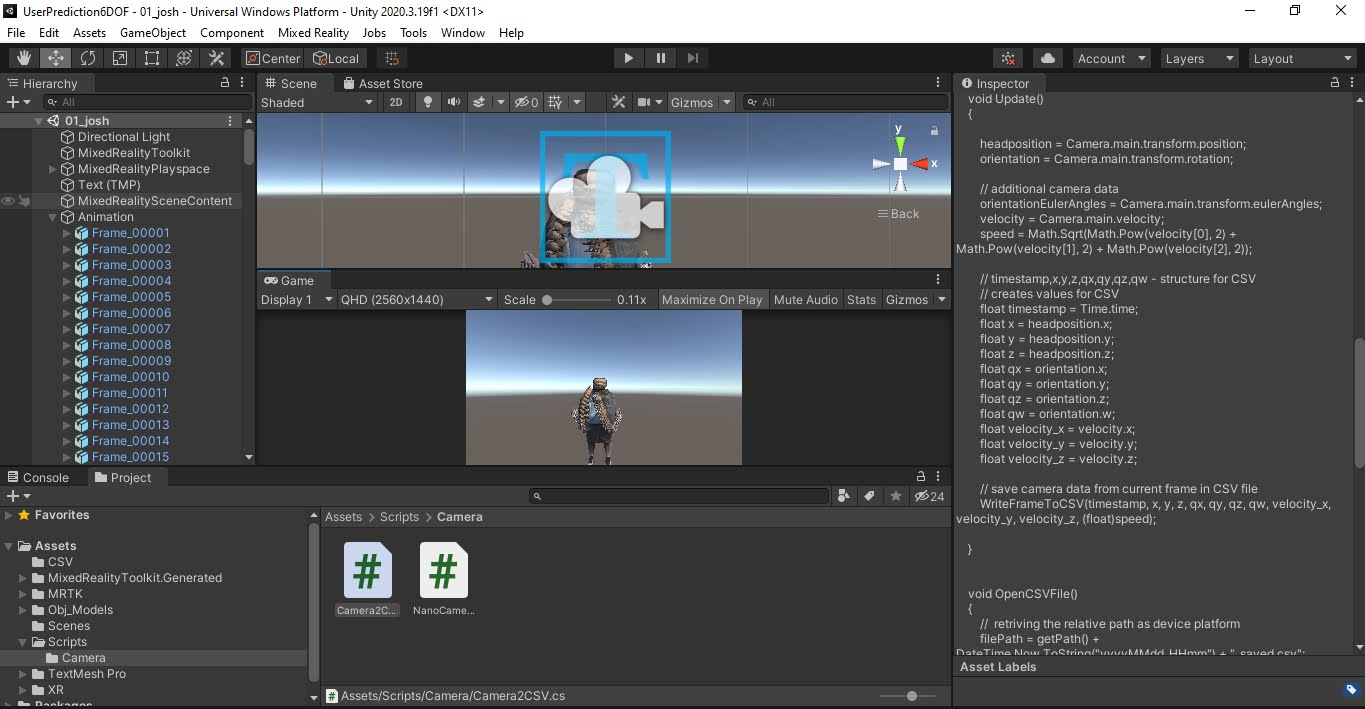
\includegraphics[width=1\textwidth, keepaspectratio]{gfx/unity.jpeg}
		\caption{\label{fig:unity} Unity 3D UserPrediction6DOF Project with placed obj-animation, underlying code and scene.}
	\end{center}
\end{figure}
\begin{wrapfigure}{L}{0.50\textwidth}
	\centering
	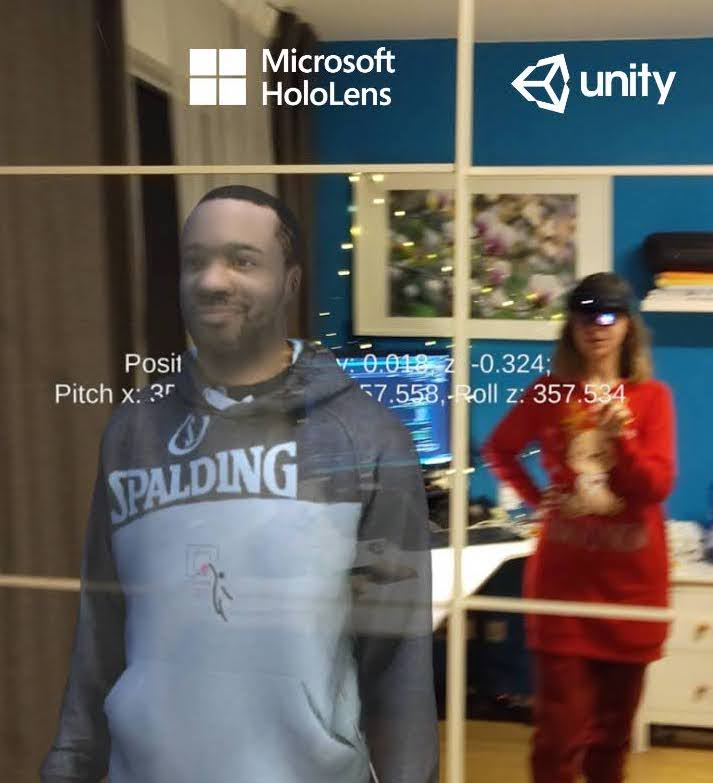
\includegraphics[width=0.48\textwidth]{gfx/josh.jpeg}
	\caption{\label{fig:josh}Photo made by Hololens 2 camera during the Unity Application running on HMD with the volumetric animated object.}
\end{wrapfigure}

As this research aims to find an approach to reduce the M2P latency during rendering and delivering the volumetric content to end-user device, the volumetric animated object was placed three meters ahead of the user in Unity application. Fig. \ref{fig:josh} presents the photo made in mirror by HoloLens camera with placed HMD on master thesis author's head. The volumetric object placed in the room between author and a mirror in the room and Fig. \ref{fig:josh} shows what author saw at that time on the HoloLens screen. Users wearing HMD thus were asked to look on animated volumetric object and to move freely inside the laboratory space. Animation frames of VV object are saved as an $obj$-files and contain information about the geometry of 3D objects. $obj$ file allows color and texture information to store in an associated file format called the Material Template Library (MTL). Multi-color geometric models render using these two files together. $obj$-files are not supporting animation. The animation of the VV object to in order to create an imitation of placed VV in VR environment was quite challenging during programming in Unity. Finally, volumetric animation object created programmatically with a loop that cycles through each individual frame with the corresponding mesh and calculated speed to give the user the experience of a real volumetric video.

User position and rotation data are logged in $csv$-file. This raw data has been converted into datasets on the preprocessing step described in section \ref{sec:impl:dataset:preprocessing} and thus original interpolated dataset, the transformed with flipped negative quaternions and several normalised datasets were used in experiments during model development and hyperparameters search.

%#######################################

\subsubsection{Training and evaluation}
\label{sec:impl:model:dev:programming}
All evaluated models are implemented in Python with Python-native framework PyTorch. After model with the inner layered structure was initialized using tensor input and output size, the training loop need to be explicit implemented in PyTorch. 

The main components of training loop are the model itself, the loss function, and the optimiser. Models creation are described in section \ref{sec:impl:model}. PyTorch's loss function $MSELoss()$ is used for creation of criteria that help to measure the error of mean squared format that is squared L2 normalization. It computes the average value of the squared differences that lie between the predicted and actual values. The value of $MSELoss()$ will always be a positive number, irrespective of whatever signs the predicted and actual values have. During training loop on every epoch when working with batched input, PyTorch will adjust model weight parameter in such way that value of $MSELoss()$ tends to be 0.00

PyTorch's optimizer is an algorithm used to change the attributes of the neural network such as weights and learning rate in order to reduce the losses. The standard optimiser is Gradient Descent used heavily in linear regression and classification algorithms. The know problem of the vanishing gradient was first discovered by Hochreiter, a German computer scientist, back in 1991 \cite{lstm_orig}. Bengio, a professor at the University of Montreal, also discovered the vanishing descent problem but a bit later – he wrote about it in 1994 \cite{rnn_difficults}. Network weights are assigned at the start of the neural network with the random values, which are close to zero, and from there the network trains them up. Briefly say, the vanishing descent problem rises from the starting weight value close to zero and repetitive multiplication of inputs $x_t, x_{t-1}, x_{t-2},...,x_{t-n}$ by this value so that mathematically gradient becomes less and less with each multiplication. The lower the gradient is, the harder it is for the network to update the weights and the longer it takes to get to the final result. Additionally, in RNN the training of current cell is based on inputs that are coming from previous untrained layers. So, because of the vanishing gradient, the whole network is not being trained properly.

Adam optimizer is the extended version of stochastic gradient descent and was first introduced in 2014. The name is derived from adaptive moment estimation and uses estimations of the first and second moments of the gradient to adapt the learning rate for each weight of the neural network. The first moment is mean, and the second moment is uncentered variance with calculated with no mean subtracted. The moments are not treated as network's parameters nor constants, they can be thought of as some intermediate results of computing the output of the layer. PyTorch's optimizer $Adam$  is used in evaluated models to reduce the training and validation losses in batches and epochs.

Training of any kind of neural network is a repetitive process, looping back and forth between forward-prop and back-prop. During each epoch in training, there are two stages: training and validation. After each training step, the network’s weights are tweaked a bit to minimize the loss function. On the validation step the current state of the model is evaluated to check if there has been any improvement after the most recent update. When two for loops are created, the $train()$ mode must be activated during training and the $eval()$ mode during the validation. With the $train()$ mode the network’s weights will to be updated in order to reduce the training loss on the next epoch, the $eval()$ mode signals the model that there is no need to calculate the gradients. The model parameter, such batch size, learning rate and weigh decay must be set correctly so that the training and validation can decreasing parallel on each epoch. Normally, on the very first epochs, the validation loss is greater than the training loss and model is unable to accurately model the predict a validation data, and hence generates higher error. During model training on every epoch the training loss and validation loss both decrease and after some amount of epochs stabilize at a specific point. The model converges upon a final solution and it is a good fit when the loss is low and stable and in this moment model's training must be stopped. It is possible to train model for a very long period so that the validation loss stops to decrease and starts to increase again. It means model is overtrained and cannot generalize on new data. Regarding the very low training loss, model produces higher error on validation test and high error on test dataset. The early stopping technique was used to prevent overfitting with stopping the training when both losses are low and stable. The early stopping algorithm is implemented manually in this thesis using Python and build in final Python application $UserPrediction6DOF$.

\subsubsection{Hyperparameter search}
\label{sec:impl:model:dev:search}
Model's training and validation loss are calculated on every epoch and in best case must decrease parallel every epoch and stabilize on very low point. The model hyperparameters influences the training process and can drastically change the final result, leading to overfitted, underfitted or successfully learned model. Hyperparameters are the variables which determines the network structure or how the network is trained. In this master thesis the following hyperparameters must be tuned: the number of hidden layers, optimizer's learning rate, weight decay, batch size, and number of epochs. For example, the learning rate of Adam optimiser is a hyperparameter because it is set before model see the the training data. On the other hand, the weights of a neural network and the first and second moments of the Adam's gradient are not its hyperparameters because they are trained and modified during training loop.

For the hyperparameter tune the grid search is applied. Grid search is a process that searches exhaustively through a manually specified subset of the hyperparameter space of the evaluated model. Every training of the model during 500 epochs on 6-DoF dataset takes on CPU up to 2 hours with up to 95\% of CPU usage. The grid for the exhaustive search is created with Bash-script that sets $hidden-dim$ and $batch-size$ in the loop to be equal power of two; $lr-adam$ and $lr-multiplicator$ are float numbers with a floating-point step. 

The hyperparameters search is done using VCA GPU cluster which is installed with the $SLURM$ resource manager/scheduler for GPU based HPC (High Performance Computing). $Singularity$ container is similar to a light-weight Virtual Machine is used to containerize the application with the required environment and software stack and submit the container to run as a job in the cluster. Using VCA GPU the computation time for every job (one model training with one set of hyperparameters) is reduced from 2 hours to 15 minutes. For every evaluated model in average over hundred jobs were launched for the initial hyperparameters search and few dozens for parameter tuning. With $export$ command hyperparameters can be set with Bash as environment variables and with $nohup$ all of jobs can be scheduled for computation with preventing the jobs from being aborted automatically if the connection to the remote machine is closed. The $UserPrediction6DOF$ application detects whether a parallel computing platform $cuda$ is available and if it is a case then reads the model parameters from environment variables. The result of every job arrives as $tar$-archive with all written out-files. Therefore Bash script is created for automatically opening of hundreds archives, finding the evaluation metrics and merging the result in one log-file for future analyse and visualisation purposes.   